%-----------------------------------------------------------------------------------------
% Autor dieser Vorlage:
% Stefan Macke (http://fachinformatiker-anwendungsentwicklung.net)
% Permalink zur Vorlage: http://fiae.link/LaTeXVorlageFIAE
%
% Sämtliche verwendeten Abbildungen, Tabellen und Listings stammen von Dirk Grashorn.
%
% Lizenz: Creative Commons 4.0 Namensnennung - Weitergabe unter gleichen Bedingungen
% -----------------------------------------------------------------------------------------
 
\documentclass[
	ngerman,
	toc=listof, % Abbildungsverzeichnis sowie Tabellenverzeichnis in das Inhaltsverzeichnis aufnehmen
	toc=bibliography, % Literaturverzeichnis in das Inhaltsverzeichnis aufnehmen
	footnotes=multiple, % Trennen von direkt aufeinander folgenden Fußnoten
	parskip=half, % vertikalen Abstand zwischen Absätzen verwenden anstatt horizontale Einrückung von Folgeabsätzen
	numbers=noendperiod % Den letzten Punkt nach einer Nummerierung entfernen (nach DIN 5008)
]{scrartcl}
\pdfminorversion=5 % erlaubt das Einfügen von pdf-Dateien bis Version 1.7, ohne eine Fehlermeldung zu werfen (keine Garantie für fehlerfreies Einbetten!)
\usepackage[utf8]{inputenc} % muss als erstes eingebunden werden, da Meta/Packages ggfs. Sonderzeichen enthalten


% !TEX root = Projektdokumentation.tex

% Hinweis: der Titel muss zum Inhalt des Projekts passen und den zentralen Inhalt des Projekts deutlich herausstellen
\newcommand{\titel}{Website-Relaunch der Tourismusregion Waginger See}
\newcommand{\untertitel}{Responsive Website inklusiver Integration und Anpassung
des CMS conTRANCE}
\newcommand{\kompletterTitel}{\titel{} -- \untertitel}

\newcommand{\autorName}{Andreas Seifert}
\newcommand{\autorAnschrift}{Im Angerl 12}
\newcommand{\autorOrt}{83435 Bad Reichenhall}

\newcommand{\betriebLogo}{Bilder/waging-logo.pdf}
\newcommand{\betriebName}{makrohaus AG\xspace} 
\newcommand{\betriebAnschrift}{Getreidegasse 9}
\newcommand{\betriebOrt}{83435 Bad Reichenhall} 
 
\newcommand{\ausbildungsberuf}{Fachinformatiker für Anwendungsentwicklung}
\newcommand{\betreff}{Dokumentation zur betrieblichen Projektarbeit}
\newcommand{\pruefungstermin}{Sommer 2016}
\newcommand{\abgabeOrt}{xxxxxxxxxxx}
\newcommand{\abgabeTermin}{xxxxxxxxxxxxxxxxx}

\newcommand{\ct}{conTRANCE\xspace}
\newcommand{\kunde}{Tourist-Info Waginger See\xspace}
\newcommand{\mh}{\betriebName}
 % Metadaten zu diesem Dokument (Autor usw.)
% !TEX root = ../Projektdokumentation.tex

% Anpassung an Landessprache ---------------------------------------------------
\usepackage{babel}

% Umlaute ----------------------------------------------------------------------
%   Umlaute/Sonderzeichen wie äüöß direkt im Quelltext verwenden (CodePage).
%   Erlaubt automatische Trennung von Worten mit Umlauten.
% ------------------------------------------------------------------------------
\usepackage[T1]{fontenc}
\usepackage{textcomp} % Euro-Zeichen etc.

% Schrift ----------------------------------------------------------------------
\usepackage{lmodern} % bessere Fonts
\usepackage{relsize} % Schriftgröße relativ festlegen

% Tabellen ---------------------------------------------------------------------
\PassOptionsToPackage{table}{xcolor}
\usepackage{tabularx}
% für lange Tabellen
\usepackage{longtable}
\usepackage{array}
\usepackage{ragged2e}
\usepackage{lscape}
\newcolumntype{w}[1]{>{\raggedleft\hspace{0pt}}p{#1}} % Spaltendefinition rechtsbündig mit definierter Breite

% Grafiken ---------------------------------------------------------------------
\usepackage[dvips,final]{graphicx} % Einbinden von JPG-Grafiken ermöglichen
\usepackage{graphics} % keepaspectratio
\usepackage{floatflt} % zum Umfließen von Bildern
\graphicspath{{Bilder/}} % hier liegen die Bilder des Dokuments

% Sonstiges --------------------------------------------------------------------
\usepackage[titles]{tocloft} % Inhaltsverzeichnis DIN 5008 gerecht einrücken
\usepackage{amsmath,amsfonts} % Befehle aus AMSTeX für mathematische Symbole
\usepackage{enumitem} % anpassbare Enumerates/Itemizes
\usepackage{xspace} % sorgt dafür, dass Leerzeichen hinter parameterlosen Makros nicht als Makroendezeichen interpretiert werden

\usepackage{makeidx} % für Index-Ausgabe mit \printindex
\usepackage[printonlyused]{acronym} % es werden nur benutzte Definitionen aufgelistet

% Einfache Definition der Zeilenabstände und Seitenränder etc.
\usepackage{setspace}
\usepackage{geometry}

% Symbolverzeichnis
\usepackage[intoc]{nomencl}
\let\abbrev\nomenclature
\renewcommand{\nomname}{Abkürzungsverzeichnis}
\setlength{\nomlabelwidth}{.25\hsize}
\renewcommand{\nomlabel}[1]{#1 \dotfill}
\setlength{\nomitemsep}{-\parsep}

\usepackage{varioref} % Elegantere Verweise. „auf der nächsten Seite“
\usepackage{url} % URL verlinken, lange URLs umbrechen etc.

\usepackage{chngcntr} % fortlaufendes Durchnummerieren der Fußnoten
% \usepackage[perpage]{footmisc} % Alternative: Nummerierung der Fußnoten auf jeder Seite neu

\usepackage{ifthen} % bei der Definition eigener Befehle benötigt
\usepackage{todonotes} % definiert u.a. die Befehle \todo und \listoftodos
\usepackage[square]{natbib} % wichtig für korrekte Zitierweise

% PDF-Optionen -----------------------------------------------------------------
\usepackage{pdfpages}
\pdfminorversion=5 % erlaubt das Einfügen von pdf-Dateien bis Version 1.7, ohne eine Fehlermeldung zu werfen (keine Garantie für fehlerfreies Einbetten!)
\usepackage[
    bookmarks,
    bookmarksnumbered,
    bookmarksopen=true,
    bookmarksopenlevel=1,
    colorlinks=true,
% diese Farbdefinitionen zeichnen Links im PDF farblich aus
    linkcolor=AOBlau, % einfache interne Verknüpfungen
    anchorcolor=AOBlau,% Ankertext
    citecolor=AOBlau, % Verweise auf Literaturverzeichniseinträge im Text
    filecolor=AOBlau, % Verknüpfungen, die lokale Dateien öffnen
    menucolor=AOBlau, % Acrobat-Menüpunkte
    urlcolor=AOBlau,
% diese Farbdefinitionen sollten für den Druck verwendet werden (alles schwarz)
    %linkcolor=black, % einfache interne Verknüpfungen
    %anchorcolor=black, % Ankertext
    %citecolor=black, % Verweise auf Literaturverzeichniseinträge im Text
    %filecolor=black, % Verknüpfungen, die lokale Dateien öffnen
    %menucolor=black, % Acrobat-Menüpunkte
    %urlcolor=black,
%
    %backref, % Quellen werden zurück auf ihre Zitate verlinkt
    pdftex,
    plainpages=false, % zur korrekten Erstellung der Bookmarks
    pdfpagelabels=true, % zur korrekten Erstellung der Bookmarks
    hypertexnames=false, % zur korrekten Erstellung der Bookmarks
    linktocpage % Seitenzahlen anstatt Text im Inhaltsverzeichnis verlinken
]{hyperref}
% Befehle, die Umlaute ausgeben, führen zu Fehlern, wenn sie hyperref als Optionen übergeben werden
\hypersetup{
    pdftitle={\titel -- \untertitel},
    pdfauthor={\autorName},
    pdfcreator={\autorName},
    pdfsubject={\titel -- \untertitel},
    pdfkeywords={\titel -- \untertitel},
}


% zum Einbinden von Programmcode -----------------------------------------------
\usepackage{listings}
\usepackage{xcolor}
\definecolor{hellgelb}{rgb}{1,1,0.9}
\definecolor{colKeys}{rgb}{0,0,1}
\definecolor{colIdentifier}{rgb}{0,0,0}
\definecolor{colComments}{rgb}{0,0.5,0}
\definecolor{colString}{rgb}{1,0,0}
\lstset{
    float=hbp,
	basicstyle=\footnotesize,
    identifierstyle=\color{colIdentifier},
    keywordstyle=\color{colKeys},
    stringstyle=\color{colString},
    commentstyle=\color{colComments},
    backgroundcolor=\color{hellgelb},
    columns=flexible,
    tabsize=2,
    frame=single,
    extendedchars=true,
    showspaces=false,
    showstringspaces=false,
    numbers=left,
    numberstyle=\tiny,
    breaklines=true,
    breakautoindent=true,
	captionpos=b,
}
\lstdefinelanguage{cs}{
	sensitive=false,
	morecomment=[l]{//},
	morecomment=[s]{/*}{*/},
	morestring=[b]",
	morekeywords={
		abstract,event,new,struct,as,explicit,null,switch
		base,extern,object,this,bool,false,operator,throw,
		break,finally,out,true,byte,fixed,override,try,
		case,float,params,typeof,catch,for,private,uint,
		char,foreach,protected,ulong,checked,goto,public,unchecked,
		class,if,readonly,unsafe,const,implicit,ref,ushort,
		continue,in,return,using,decimal,int,sbyte,virtual,
		default,interface,sealed,volatile,delegate,internal,short,void,
		do,is,sizeof,while,double,lock,stackalloc,
		else,long,static,enum,namespace,string},
}
\lstdefinelanguage{natural}{
	sensitive=false,
	morecomment=[l]{/*},
	morestring=[b]",
	morestring=[b]',
	alsodigit={-,*},
	morekeywords={
		DEFINE,DATA,LOCAL,END-DEFINE,WRITE,CALLNAT,PARAMETER,USING,
		IF,NOT,END-IF,ON,*ERROR-NR,ERROR,END-ERROR,ESCAPE,ROUTINE,
		PERFORM,SUBROUTINE,END-SUBROUTINE,CONST,END-FOR,END,FOR,RESIZE,
		ARRAY,TO,BY,VALUE,RESET,COMPRESS,INTO,EQ},
}
\lstdefinelanguage{php}{
	sensitive=false,
	morecomment=[l]{/*},
	morestring=[b]",
	morestring=[b]',
	alsodigit={-,*},
	morekeywords={
		abstract,and,array,as,break,case,catch,cfunction,class,clone,const,
		continue,declare,default,do,else,elseif,enddeclare,endfor,endforeach,
		endif,endswitch,endwhile,extends,final,for,foreach,function,global,
		goto,if,implements,interface,instanceof,namespace,new,old_function,or,
		private,protected,public,static,switch,throw,try,use,var,while,xor
		die,echo,empty,exit,eval,include,include_once,isset,list,require,
		require_once,return,print,unset},
}
 % verwendete Packages
% !TEX root = ../Projektdokumentation.tex

% Seitenränder -----------------------------------------------------------------
\setlength{\topskip}{\ht\strutbox} % behebt Warnung von geometry
\geometry{a4paper,left=20mm,right=20mm,top=25mm,bottom=35mm}

\usepackage[
	automark, % Kapitelangaben in Kopfzeile automatisch erstellen
	headsepline, % Trennlinie unter Kopfzeile
	ilines % Trennlinie linksbündig ausrichten
]{scrpage2}
\usepackage{multicol}
% Kopf- und Fußzeilen ----------------------------------------------------------
\pagestyle{scrheadings}
% chapterpagestyle gibt es nicht in scrartcl
%\renewcommand{\chapterpagestyle}{scrheadings}
\clearscrheadfoot

% Kopfzeile
\renewcommand{\headfont}{\normalfont} % Schriftform der Kopfzeile
\ihead{\large{\textsc{\titel}}\\ \small{\untertitel} \\[2ex] \textit{\headmark}}
\chead{}
\ohead{\includegraphics[scale=0.5, trim=0 0 0 1cm]{\betriebLogo}}
\setlength{\headheight}{15mm} % Höhe der Kopfzeile
%\setheadwidth[0pt]{textwithmarginpar} % Kopfzeile über den Text hinaus verbreitern (falls Logo den Text überdeckt)

% Fußzeile
\ifoot{\autorName}
\cfoot{}
\ofoot{\pagemark}

% Überschriften nach DIN 5008 in einer Fluchtlinie
% ------------------------------------------------------------------------------

% Abstand zwischen Nummerierung und Überschrift definieren
% > Schön wäre hier die dynamische Berechnung des Abstandes in Abhängigkeit
% > der Verschachtelungstiefe des Inhaltsverzeichnisses
\newcommand{\headingSpace}{1.5cm}

% Abschnittsüberschriften im selben Stil wie beim Inhaltsverzeichnis einrücken
\renewcommand*{\othersectionlevelsformat}[3]{
  \makebox[\headingSpace][l]{#3\autodot}
}

% Für die Einrückung wird das Paket tocloft benötigt
%\cftsetindents{chapter}{0.0cm}{\headingSpace}
\cftsetindents{section}{0.0cm}{\headingSpace}
\cftsetindents{subsection}{0.0cm}{\headingSpace}
\cftsetindents{subsubsection}{0.0cm}{\headingSpace}
\cftsetindents{figure}{0.0cm}{\headingSpace}
\cftsetindents{table}{0.0cm}{\headingSpace}


% Allgemeines
% ------------------------------------------------------------------------------

\onehalfspacing % Zeilenabstand 1,5 Zeilen
\frenchspacing % erzeugt ein wenig mehr Platz hinter einem Punkt

% Schusterjungen und Hurenkinder vermeiden
\clubpenalty = 10000
\widowpenalty = 10000
\displaywidowpenalty = 10000

% Quellcode-Ausgabe formatieren
\lstset{numbers=left, numberstyle=\tiny, numbersep=5pt, breaklines=true}
\lstset{emph={square}, emphstyle=\color{red}, emph={[2]root,base}, emphstyle={[2]\color{blue}}}

\counterwithout{footnote}{section} % Fußnoten fortlaufend durchnummerieren
\setcounter{tocdepth}{\subsubsectionlevel} % im Inhaltsverzeichnis werden die Kapitel bis zum Level der subsubsection übernommen
\setcounter{secnumdepth}{\subsubsectionlevel} % Kapitel bis zum Level der subsubsection werden nummeriert

% Aufzählungen anpassen
\renewcommand{\labelenumi}{\arabic{enumi}.}
\renewcommand{\labelenumii}{\arabic{enumi}.\arabic{enumii}.}
\renewcommand{\labelenumiii}{\arabic{enumi}.\arabic{enumii}.\arabic{enumiii}}

% Tabellenfärbung:
\definecolor{heading}{rgb}{0.64,0.78,0.86}
\definecolor{odd}{rgb}{0.9,0.9,0.9}
 % Definitionen zum Aussehen der Seiten
% !TEX root = ../Projektdokumentation.tex

% Abkürzungen, ggfs. mit korrektem Leerraum
\newcommand{\bs}{$\backslash$\xspace}
\newcommand{\bspw}{bspw.\xspace}
\newcommand{\bzw}{bzw.\xspace}
\newcommand{\ca}{ca.\xspace}
\newcommand{\dahe}{\mbox{d.\,h.}\xspace}
\newcommand{\etc}{etc.\xspace}
\newcommand{\eur}[1]{\mbox{#1\,\texteuro}\xspace}
\newcommand{\evtl}{evtl.\xspace}
\newcommand{\ggfs}{ggfs.\xspace}
\newcommand{\Ggfs}{Ggfs.\xspace}
\newcommand{\gqq}[1]{\glqq{}#1\grqq{}}
\newcommand{\inkl}{inkl.\xspace}
\newcommand{\insb}{insb.\xspace}
\newcommand{\ua}{\mbox{u.\,a.}\xspace}
\newcommand{\usw}{usw.\xspace}
\newcommand{\Vgl}{Vgl.\xspace}
\newcommand{\zB}{\mbox{z.\,B.}\xspace} 

% Befehle für häufig anfallende Aufgaben
\newcommand{\Abbildung}[1]{\autoref{fig:#1}}
\newcommand{\Anhang}[1]{\appendixname{}~\ref{#1}: \nameref{#1} \vpageref{#1}}
\newcommand{\includegraphicsKeepAspectRatio}[2]{\includegraphics[width=#2\textwidth,height=#2\textheight,keepaspectratio]{#1}}
\newcommand{\Zitat}[2][\empty]{\ifthenelse{\equal{#1}{\empty}}{\citep{#2}}{\citep[#1]{#2}}}
\newcommand{\Autor}[1]{\textsc{#1}} % zum Ausgeben von Autoren
\newcommand{\itemd}[2]{\item{\textbf{#1}}\\{#2}} % erzeugt ein Listenelement mit fetter Überschrift

% fügt Tabellen aus einer TEX-Datei ein
\newcommand{\tabelle}[3] % Parameter: caption, label, file
{\begin{table}[htbp]
\centering
\singlespacing
\input{Tabellen/#3}
\caption{#1}
\label{#2}
\end{table}}

\newcommand{\tabelleAnhang}[1] % Parameter: file
{\begin{center}
\singlespacing
\input{Tabellen/#1}
\end{center}}

% einfaches Wechseln der Schrift, z.B.: \changefont{cmss}{sbc}{n}
\newcommand{\changefont}[3]{\fontfamily{#1} \fontseries{#2} \fontshape{#3} \selectfont}

% Verwendung analog zu \includegraphics
\newlength{\myx} % Variable zum Speichern der Bildbreite
\newlength{\myy} % Variable zum Speichern der Bildhöhe
\newcommand\includegraphicstotab[2][\relax]{%
% Abspeichern der Bildabmessungen
\settowidth{\myx}{\includegraphics[{#1}]{#2}}%
\settoheight{\myy}{\includegraphics[{#1}]{#2}}%
% das eigentliche Einfügen
\parbox[c][1.1\myy][c]{\myx}{%
\includegraphics[{#1}]{#2}}%
}

\definecolor{AOBlau}{rgb}{0, 0.28, 0.56}

% verschiedene Befehle um Wörter semantisch auszuzeichnen ----------------------
\newcommand{\Index}[2][\empty]{\ifthenelse{\equal{#1}{\empty}}{\index{#2}#2}{\index{#1}#2}}
\newcommand{\Fachbegriff}[2][\empty]{\ifthenelse{\equal{#1}{\empty}}{\textit{\Index{#2}}}{\textit{\Index[#1]{#2}}}}
\newcommand{\NeuerBegriff}[2][\empty]{\ifthenelse{\equal{#1}{\empty}}{\textbf{\Index{#2}}}{\textbf{\Index[#1]{#2}}}}

\newcommand{\Ausgabe}[1]{\texttt{#1}}
\newcommand{\Eingabe}[1]{\texttt{#1}}
\newcommand{\Code}[1]{\texttt{#1}}
\newcommand{\Datei}[1]{\texttt{#1}}

\newcommand{\Assembly}[1]{\textsf{#1}}
\newcommand{\Klasse}[1]{\textsf{#1}}
\newcommand{\Methode}[1]{\textsf{#1}}
\newcommand{\Attribut}[1]{\textsf{#1}}

\newcommand{\Datentyp}[1]{\textsf{#1}}
\newcommand{\XMLElement}[1]{\textsf{#1}}
\newcommand{\Webservice}[1]{\textsf{#1}}

\newcommand{\Refactoring}[1]{\Fachbegriff{#1}}
\newcommand{\CodeSmell}[1]{\Fachbegriff{#1}}
\newcommand{\Metrik}[1]{\Fachbegriff{#1}}
\newcommand{\DesignPattern}[1]{\Fachbegriff{#1}}
 % eigene allgemeine Befehle, die z.B. die Arbeit mit LaTeX erleichtern
% Tabellen, die den Zwischenstand nach einer Projektphase verdeutlichen
\newcommand{\Zwischenstand}[2]{\subsection{Zwischenstand}Tabelle~\ref{tab:#2} zeigt den Zwischenstand nach der #1.\tabelle{Zwischenstand nach der #1}{tab:#2}{#2.tex}}

% Abkürzungen
\newcommand{\Versis}{\textsc{Versis}\xspace}
\newcommand{\NI}{NatInfo\xspace}
\newcommand{\AO}{\textsc{Alte Oldenburger} Krankenversicherung\xspace}
 % eigene projektspezifische Befehle, z.B. Abkürzungen usw.
\usepackage{pdfpages} 
\usepackage{upquote}
\usepackage{listings}
\usepackage{color}
\begin{document}

% kann nach dem Lesen entfernt werden ---------------------------------------
\pagestyle{plain}
% !TEX root = Projektdokumentation.tex
\section*{Über diese Vorlage}

Diese \LaTeX-Vorlage wurde von Stefan Macke\footnote{Blog des Autors:
\url{http://fachinformatiker-anwendungsentwicklung.net}, Twitter:
\Eingabe{@StefanMacke}} als Grundlage für die Projektdokumentationen der Auszubildenden zum Fachinformatiker mit Fachrichtung
Anwendungsentwicklung bei der \AO entwickelt. Nichtsdestotrotz dürfte sie ebenso für die anderen IT-Berufe\footnote{\zB IT-Kaufleute, Fachinformatiker
mit Fachrichtung Systemintegration \usw} geeignet sein, da diese anhand der gleichen Verordnung bewertet werden.

Diese Vorlage enthält bereits eine Vorstrukturierung der möglichen Inhalte einer tatsächlichen Projektdokumentation, die auf Basis der
Erfahrungen im Rahmen der Prüfertätigkeit des Autors erstellt und unter Zuhilfenahme von \citet{Rohrer2011} abgerundet wurden.

Sämtliche verwendeten Abbildungen, Tabellen und Listings stammen von \citet{Grashorn2010}.

Download-Link für diese Vorlage: \url{http://fiae.link/LaTeXVorlageFIAE}

Auch verfügbar auf GitHub: \url{https://github.com/StefanMacke/latex-vorlage-fiae}

\subsection*{Lizenz}

\begin{center}
\includegraphicsKeepAspectRatio{CC-Logo.pdf}{0.3}
\end{center}
Dieses Werk steht unter einer Creative Commons Namensnennung - Weitergabe unter gleichen Bedingungen 4.0 International Lizenz.
\footnote{\url{http://creativecommons.org/licenses/by-sa/4.0/}}

\begin{center}
\includegraphicsKeepAspectRatio{CC-Attribution.pdf}{0.07}
\includegraphicsKeepAspectRatio{CC-ShareAlike.pdf}{0.07}
\end{center}

\begin{description}
	\item[Namensnennung] Sie müssen den Namen des Autors/Rechteinhabers in der von ihm festgelegten Weise nennen.
	\footnote{Die Namensnennung im \LaTeX-Quelltext mit Link auf \url{http://fiae.link/LaTeXVorlageFIAE} reicht hierfür aus.}
	\item[Weitergabe unter gleichen Bedingungen] Wenn Sie das lizenzierte Werk \bzw den lizenzierten Inhalt bearbeiten
	oder in anderer Weise erkennbar als Grundlage für eigenes Schaffen verwenden, dürfen Sie die daraufhin neu entstandenen
	Werke \bzw Inhalte nur unter Verwendung von Lizenzbedingungen weitergeben, die mit denen dieses Lizenzvertrages identisch oder vergleichbar sind.
\end{description}

\subsection*{Inhalt der Projektdokumentation}

Grundsätzlich definiert die \citet[S.~1746]{Bundesgesetzblatt48}\footnote{Dieses
Dokument sowie alle weiteren hier genannten können unter
\url{http://fiae.link/LaTeXVorlageFIAEQuellen} heruntergeladen werden.} das Ziel der Projektdokumentation wie folgt:
\begin{quote}
"`Durch die Projektarbeit und deren Dokumentation soll der Prüfling belegen, daß er Arbeitsabläufe und Teilaufgaben zielorientiert unter
Beachtung wirtschaftlicher, technischer, organisatorischer und zeitlicher Vorgaben selbständig planen und kundengerecht umsetzen sowie
Dokumentationen kundengerecht anfertigen, zusammenstellen und modifizieren kann."'
\end{quote}

Und das \citet[S.~36]{BMBF2000} ergänzt:
\begin{quote}
"`Die Ausführung der Projektarbeit wird mit praxisbezogenen Unterlagen dokumentiert.
Der Prüfungsausschuss bewertet die Projektarbeit anhand der Dokumentation. Dabei
wird nicht das Ergebnis -- \zB ein lauffähiges Programm -- herangezogen, sondern
der Arbeitsprozess. Die Dokumentation ist keine wissenschaftliche Abhandlung,
sondern eine handlungsorientierte Darstellung des Projektablaufs mit
praxisbezogenen, d.h. betriebüblichen Unterlagen. Sie soll einen Umfang von
maximal 10 bis 15 DIN A 4-Seiten nicht überschreiten. Soweit erforderlich können in
einem Anhang \zB den Zusammenhang erläuternde Darstellungen beigefügt werden."'
\end{quote}

Außerdem werden dort die grundlegenden Inhalte der Projektdokumentation aufgelistet:
\begin{itemize}
	\item Name und Ausbildungsberuf des Prüfungsteilnehmers
	\item Angabe des Ausbildungsbetriebes
	\item Thema der Projektarbeit
	\item Falls erforderlich, Beschreibung/Konkretisierung des Auftrages
	\item Umfassende Beschreibung der Prozessschritte und der erzielten Ergebnisse
	\item Gegebenenfalls Veränderungen zum Projektantrag mit Begründung
	\item Wenn für das Projekt erforderlich, ein Anhang mit praxisbezogenen Unterlagen und Dokumenten. Dieser Anhang sollte nicht
	aufgebläht werden. Die angehängten Dokumente und Unterlagen sind auf das absolute Minimum zu beschränken.
\end{itemize}

In den folgenden Kapiteln werden diese geforderten Inhalte und sinnvolle Ergänzungen nun meist stichwortartig und \ggfs mit
Beispielen beschrieben. Nicht alle Kapitel müssen in jeder Dokumentation vorhanden sein. Handelt es sich \bspw um ein in sich
geschlossenes Projekt, kann das Kapitel~\ref{sec:Projektabgrenzung}: \nameref{sec:Projektabgrenzung} entfallen; arbeitet die
Anwendung nur mit \acs{XML}-Dateien, kann und muss keine Datenbank beschrieben werden \usw


\subsection*{Formale Vorgaben}

Die formalen Vorgaben zum Umfang und zur Gestaltung der Projektdokumentation können je nach IHK recht unterschiedlich sein.
Normalerweise sollte die zuständige IHK einen Leitfaden bereitstellen, in dem alle Formalien nachgelesen werden können,
wie \zB bei der \citet{MerkblattIHK}.

Als Richtwert verwende ich 15 Seiten für den reinen Inhalt. Also in dieser Vorlage alle Seiten, die arabisch nummeriert
sind (ohne das Literaturverzeichnis und die eidesstattliche Erklärung).
Große Abbildungen, Quelltexte, Tabellen \usw gehören in den Anhang, der 25 Seiten nicht überschreiten sollte.

Typographische Konventionen, Seitenränder \usw können in der Datei \Datei{Seitenstil.tex} beliebig angepasst werden.


\subsection*{Bewertungskriterien}
Die Bewertungskriterien für die Benotung der Projektdokumentation sind recht einheitlich und können leicht in Erfahrung
gebracht werden, \zB bei der \citet{BewertungsmatrikIHK}.
Grundsätzlich sollte die Projektdokumentation nach der Fertigstellung noch einmal im Hinblick auf diese Kriterien durchgeschaut werden.

\cleardoublepage 
\pagestyle{scrheadings}
% ---------------------------------------------------------------------------


\phantomsection
\thispagestyle{plain}
\pdfbookmark[1]{Deckblatt}{deckblatt} 
% !TEX root = Projektdokumentation.tex
\begin{titlepage}

\begin{center}

\includegraphics[scale=0.25]{LogoIHK.pdf}\\[1ex]
\Large{Abschlussprüfung \pruefungstermin}\\[3ex]

\Large{\ausbildungsberuf}\\
\LARGE{\betreff}\\[4ex]

\huge{\textbf{\titel}}\\[1.5ex]
\Large{\textbf{\untertitel}}\\[3ex]

\normalsize
Abgabetermin: \abgabeOrt, den \abgabeTermin\\[2em]
\textbf{Prüfungsbewerber:}\\
\autorName\\
\autorAnschrift\\
\autorOrt\\[5ex]

\includegraphics[scale=0.3]{\betriebLogo}\\[2ex]
\textbf{Ausbildungsbetrieb:}\\
\betriebName\\
\betriebAnschrift\\
\betriebOrt\\[5em]
\end{center}

\small
\noindent
\newline
\newline
Dieses Werk einschließlich seiner Teile ist \textbf{urheberrechtlich geschützt}.
Jede Verwertung außerhalb der engen Grenzen des Urheberrechtgesetzes ist ohne
Zustimmung des Autors unzulässig und strafbar. Das gilt insbesondere für
Vervielfältigungen, Übersetzungen, Mikroverfilmungen sowie die Einspeicherung
und Verarbeitung in elektronischen Systemen.

\end{titlepage}
\cleardoublepage

% Preface --------------------------------------------------------------------
\phantomsection
\pagenumbering{Roman}
\pdfbookmark[1]{Inhaltsverzeichnis}{inhalt}
\tableofcontents
\cleardoublepage

\phantomsection
\listoffigures
\cleardoublepage

\phantomsection
\listoftables
\cleardoublepage

\phantomsection
\lstlistoflistings
\cleardoublepage

\newcommand{\abkvz}{Abkürzungsverzeichnis}
\renewcommand{\nomname}{\abkvz}
\section*{\abkvz}
\markboth{\abkvz}{\abkvz}
\addcontentsline{toc}{section}{\abkvz}
% !TEX root = Projektdokumentation.tex

% Es werden nur die Abkürzungen aufgelistet, die mit \ac definiert und auch benutzt wurden. 
%
% \acro{VERSIS}{Versicherungsinformationssystem\acroextra{ (Bestandsführungssystem)}}
% Ergibt in der Liste: VERSIS Versicherungsinformationssystem (Bestandsführungssystem)
% Im Text aber: \ac{VERSIS} -> Versicherungsinformationssystem (VERSIS)

% Hinweis: allgemein bekannte Abkürzungen wie z.B. bzw. u.a. müssen nicht ins Abkürzungsverzeichnis aufgenommen werden
% Hinweis: allgemein bekannte IT-Begriffe wie Datenbank oder Programmiersprache müssen nicht erläutert werden,
%          aber ggfs. Fachbegriffe aus der Domäne des Prüflings (z.B. Versicherung)

% Die Option (in den eckigen Klammern) enthält das längste Label oder
% einen Platzhalter der die Breite der linken Spalte bestimmt.
\begin{acronym}[WWWWW]
	\acro{CSS}{Cascading Style Sheets}
	\acro{EPK}{Ereignisgesteuerte Prozesskette}
	\acro{HTTP}{Hypertext Transfer Protocol}
	\acro{ERM}{En\-ti\-ty-Re\-la\-tion\-ship-Mo\-dell}
	\acro{HTML}{Hypertext Markup Language}\acused{HTML}	
	\acro{IDE}{Integrated Development Environment}
	\acro{MVC}[MVC]{Model View Controller}	
	\acro{PHP}{Hypertext Preprocessor}		
	\acro{SQL}{Structured Query Language}  
	\acro{GIT}{Software zur Versionsverwaltung?????} 
	\acro{UML}{Unified Modeling Language}	
	\acro{CMS}{Content Managment System} 
	\acro{LESS}{Vereinfachte Stylesheet Sprache????}
	\acro{BEM}{Block-Element-Modifier}
	\acro{RWD}{Responsive Webdesign}
	\acro{SEO}{Search Engine Optimization}
	\acro{SVG}{Scalable Vector Graphics}
	\acro{DRY}{Don’t repeat yourself}
	\acro{CoC}{Convention over Configuration }
\end{acronym}

\clearpage

% Inhalt ---------------------------------------------------------------------
\pagenumbering{arabic}
% !TEX root = Projektdokumentation.tex
% !TEX root = ../Projektdokumentation.tex
\section{Einleitung}
\label{sec:Einleitung}
TEXT\ldots LaTeX

\subsection{Projektumfeld} 
\label{sec:Projektumfeld}
Die Firma \mh wurde von der Touristeninformation \kunde beauftragt, deren
unzeitgemäßen Internetauftritt mithilfe eines moderneren Erscheinungsbildes in
Form eines Relaunch zu erneuern. Dazu wurde das Screendesign von einer
externen Werbeagentur bereitgestellt.

Die \mh mit Sitz in Bad Reichenhall ist eine crossmedia Werbeagentur, 
die seit 2001 besteht und mittlerweile über 30 Mitarbeiter beschäftigt. 
Die Agentur unterteilt sich in die vier
Abteilungen: Projektmanagement, Kreation- und Design, Web-Technologie \& Design
sowie IT Services. Unter anderem durch die geografische Lage des Unternehmens 
begründet hat die Agentur ihren Schwerpunkt im Bereich Destinationstourismus.
Dementsprechend sind die meisten Softwarelösungen, die die \mh anbietet, darauf ausgelegt.
Zum Angebotsspektrum des Unternehmens gehören neben dem \ac{CMS} \ct 
auch Softwarelösungen wie digiMELDE als Online-Meldewesen Plattform, makroCARD
für Customer Loyality Management und ein innovatives Werkzeug zur
Erstellung von Gastgeberverzeichnissen -- digiAIR (\Fachbegriff{Web2Print}).


%Das \acs{CMS} \ct wird bereits von vielen großen und kleinen
%Destinationen bei der Pflege derer Webauftritten erfolgreich eingesetzt, wie
% \zB von Berchtesgadener Land Tourismus, Predigtstuhlbahn oder Alpine Welten – Der Bergführer.

\subsection{Projektziel} 
\label{sec:Projektziel}

Das Bestreben des Auftraggebers ist es, durch die neue Website dem Besucher
relevante Informationen zu bieten, Emotionen zu vermitteln, das Erfüllen
moderner Anforderungen, sowie Buchungen und Anfragen zu generieren.

Ein Hauptaugenmerk ist hierbei, eine optimale und geräteunabhängige Darstellung
im Web zu verwirklichen -- \ac{RWD}. Beim \ac{RWD} erfolgt der
grafische Aufbau der Website auf Basis der Anforderung des jeweiligen Endgerätes
auf dem die Website geöffnet wird. Die Umstellung auf \ac{RWD} führt demnach
zur einer vereinfachten und optimierten Bedienung in allen gängigen
Darstellungsgrößen. Daraus erschließt sich das Ziel eine bestmögliche
Benutzererfahrung zu schaffen.

Ein weiteres Anliegen ist die zeitaufwändige und komplizierte Einpflege von
Inhalten und weitere technische Mängel wie \zB dürftige \ac{SEO} mit einem
\ac{CMS} zu umgehen.


\subsection{Projektbegründung} 
\label{sec:Projektbegruendung}
Basierend auf der Kernzielgruppe "`50+"' ist eine übersichtliche und
anpassungsfähige Darstellung von relevanten Informationen signifikant. 
Die statische Darbietung auf verschiedenen Displaygrößen benachteiligt die
\Fachbegriff{Userability} schwerwiegend und führt dazu, dass
überdurchschnittlich viele Nutzer die Website verlassen. Durch das modernere
Erscheinungsbild in Kombination mit \ac{RWD} kann dies verhindert werden.
 
Ebenso unvorteilhaft ist die lückenhafte Suchmaschinenoptimierung, die die Suche
der Website erschwert. Hinzu kommen noch Performance- und
Sicherheitsprobleme, die durch die veraltete Technik der aktuellen Website
ausgelöst werden. Die eben genannten Hindernisse als auch die komplizierte und
zeitaufwändige Einpflege von Inhalten kann durch die Implementierung des
hauseigenen sowie modernen \ac{CMS} \ct umgangen werden.

Auf Grund dieser Lösungsansätze und die dafür nötigen Kompetenzen hat sich die
\kunde entschlossen, der Firma \mh die Entwicklung einer neuen Website in
Auftrag zu geben.

\subsection{Projektabgrenzung} 
\label{sec:Projektabgrenzung}

\xx noch zu machen

% !TEX root = ../Projektdokumentation.tex
\section{Projektplanung} 
\label{sec:Projektplanung}

\subsection{Projektphasen}
\label{sec:Projektphasen}

Für die Umsetzung des Projektes standen 70 Stunden zur Verfügung. Diese wurden vor
Beginn des Projektes auf verschiedene Phasen der Softwarentwicklung verteilt.
Die Folgende Tabelle~\ref{tab:Zeitplanung} zeigt eine grobe Planung
der Entwicklungszeit.
Eine detailliertere Zeitplanung kann im \Anhang{app:Zeitplanung} entnommen werden.
\tabelle{Grobe Zeitplanung}{tab:Zeitplanung}{ZeitplanungKurz}


\subsection{Ressourcenplanung}
\label{sec:Ressourcenplanung}
Alle im Projekt verwendeten Ressourcen werden im \Anhang{list:Ressourcenplanung}
aufgeführt. Diese werden in Soft- und Hardwareressourcen, als auch in Personal
unterteilt. Es wurden bereits vorhandene Ressourcen der \mh verwendet, um die
Kosten gering zu halten. Ansonsten wurde ausschließlich lizenzfreie Software (wie \zB
\FachBegriff{Open Source}) für das Projekt herangezogen.


\subsection{Entwicklungsprozess}
\label{sec:Entwicklungsprozess}
Da das Screendesign von einer externen Werbeagentur bereitgestellt wird, ist
ein agiler Entwicklungsprozess vonnöten. Dadurch kann man ohne großen Aufwand
und flexibel auf Änderungen seitens des Screendesigns reagieren.

Agile Softwareentwicklung zeichnet sich durch selbstorganisierende Teams, sowie eine iterative
und inkrementelle Vorgehensweise aus. Es wird versucht, mit geringem
bürokratischem Aufwand und Regeln auszukommen und sich schnell an Veränderungen anzupassen,
ohne dabei das Risiko für Fehler zu erhöhen. \footnote{Vgl. \cite{wiki:Agile_Softwareentwicklung}}

Da das Projektmanagment im ständigen Kontakt zum Kunden, als auch zur externen
Werbeagentur steht, kann ein agiler Entwicklungsprozess gewährleistet werden.

% !TEX root = ../Projektdokumentation.tex
\section{Analysephase} 
\label{sec:Analysephase}


\subsection{Ist-Analyse} 
\label{sec:IstAnalyse}

Im Verlauf der Ist-Analyse wurde eine Liste mit allen Problemen sowie
Anforderungen und deren technischen Lösungsmöglichkeiten aufgeführt. 

Derzeitig beruht die Website auf einer veralteten Version von \ct (5),
die noch einen komplizierten Ablauf zur Einpflege von Inhalten beherbergt. Dies ist mit
einem hohen Zeitaufwand sowie einer hohen Fehleranfälligkeit behaftet. Zudem
fehlen einige technischen Features, wie \zB umfangreiche \ac{SEO} und eine
Mediendatenbank zur einfachen Verwaltung von Bilddateien \oae Formaten. 
Außerdem wird die Website momentan auf allen Geräten in der Desktop-Ansicht
präsentiert, was zu einer schlechten Bedienung der Steuerelemente führt.
Möchte sich der Kunde über ein Smartphone informieren, wird er
Schwierigkeiten beim Navigieren der Website haben. 

Der mit \ac{RWD} konzeptionierte Relaunch der Website mit Anbindung der
aktuellen \ct Version (6) löst alle oben benannten technischen Probleme und hält
alle Kundenanforderungen ein.

\subsection{Wirtschaftlichkeitsanalyse}
\label{sec:Wirtschaftlichkeitsanalyse}
Aufgrund der Technischer- und \Fachbegriff{Usability}-Problemen, die in
Kapitel \ref{sec:Projektbegruendung} \nameref{sec:Projektbegruendung}
sowie \ref{sec:IstAnalyse} \nameref{sec:IstAnalyse} beschrieben werden,
ist die Entwicklung in Form eines Relaunches erforderlich. In den folgenden Abschnitten wird die Gerechtfertigung aus wirtschaftlichen Standpunkten näher
erläutert.

\subsubsection{\gqq{Make or Buy}-Entscheidung}
\label{sec:MakeOrBuyEntscheidung}
In diesem Projekt ist eine "`Make or Buy"'-Entscheidung nicht gegeben, da die
Anforderungen des Kunden \kunde in einigen Fällen zu spezifiziert sind.

\subsubsection{Projektkosten}
\label{sec:Projektkosten}

In diesem Projekt setzen sich die Kosten für die Durchführung des Projekts
nur aus Personalkosten zusammen. Zur besseren Überischt für den Kunden erfolgte
die Abrechnung über einen Mischstundensatz von 65€. Dieser Satz ergibt sich
durch den Mittelwert der Stundensätze für Projektmanagement, Design und Entwicklung.

Die Aufstellung der Kosten kann in der Tabelle~\ref{tab:Kostenaufstellung}
entnommen werden.
\tabelle{Kostenaufstellung}{tab:Kostenaufstellung}{Kostenaufstellung.tex}



\subsubsection{Amortisationsdauer}
\label{sec:Amortisationsdauer}

Aufgrund dessen, dass es sich um ein externes Projekt handelt, welches sich bei
der Bezahlung der Rechnung für die \mh bereits alle Kosten deckt (inkl. Gewinn), ist
eine Amortisationsdauer für das Unternehmen nicht notwendig.
Auf der Seite des Kunden kann eine Berechnung der Amortisierungszeit nicht exakt
durchgeführt werden, da sich der positive wirtschaftliche Effekt angesichts der
verbesserten \Fachbegriff{Usability} und der Zeiteinsparung bei der
Inhaltspflege nur sehr schlecht einschätzen lässt.


\subsection{Anwendungsfälle}
\label{sec:Anwendungsfaelle}

Die Übersicht der anfallenden Anwendungsfälle, die durch den Relaunch der
Website abgedeckt werden sollen, finden sich in Form eines Use-Case-Diagramms
im \Anhang{app:UseCase}. Es bildet die nötigen Funktionen ab, die aus Sicht
des Redakteurs \bzw Administrators sowie des herkömmlichen Benutzer unerlässlich
sind. Die zwei Aktionen "`Aufruf der Konfiguration und Rechteverwaltung"' sowie
"`Einpflege von Inhalten"' sind zusammengefasste Punkte, die theoretisch selber
Use-Case-Diagramme beherbergen.

\subsection{Qualitätsanforderungen}
\label{sec:Qualitaetsanforderungen}

Da es sich bei \ct um ein fertiges \ac{CMS} handelt, welches alle
Entwicklungsphasen bereits durchlaufen hat, sind in diesem Bezug keine
Qualitätsanforderungen vorhanden. Die im \Fachbegriff{Frontend} nötigen
Anforderungen im Hinblick auf Performance und \Fachbegriff{Usability} werden im
Folgenden erläutert.

Infolge der verschiedenen Darstellungen je nach Browser und
benutzerdefinierten Einstellungen ist eine ständige Überprüfung auf
Darstellungsfehler in der Implementierungsphase unabdingbar.
Um die Gestaltungs- und Layoutelemente reaktionsfähiger zu bilden, werden
relative Bezugsgrößen für die Maßangabe verwendet. Diese werden \zB bei
Schriftgrößen, Bildgrößen und Layout-Grids verwendet. Skalierende Icons und 
änhliche Grafiken werden zwecks der scharfen Darstellung in Form von \ac{SVG}
eingebettet.

Um eine angenehme und flüssige Bedienung am Smartphone zu gewährleisten, wird
auf Javascript falls möglich verzichtet.

\subsection{Lastenheft}
\label{sec:Lastenheft}

Die Anforderungen im Lastenheft wurden im Laufe eines ausführlichen Gespräches
mit dem Kunden vom Projektmanagement im Form eines Grobkonzeptes aufgeführt. Ein
Auszug dafür befindet sich im Anhang \ref{app:Lastenheft} auf Seite
\pageref{app:Lastenheft}.

\clearpage

% !TEX root = ../Projektdokumentation.tex
\section{Entwurfsphase} 
\label{sec:Entwurfsphase}

\subsection{Zielplattform}
\label{sec:Zielplattform}
Da es bei diesem Projekt um eine Umsetzung einer Website handelt, wird diese
Applikation auf einem externen Webserver (\ac{HTTP}, Apache2) laufen.
Dementsprechend wird mit der Skriptsprache \ac{PHP} (Version 5.5) gearbeitet. Der Inhalt der Website wird aus
einer MySQL5 Datenbank gespeist.

Neben dem HTML5 wird auch
\ac{CSS}3 und jQuery 1.11.2 -- eine Javascript-Bibliothek für die Umsetzung des
HTML-Dummys eingesetzt. Bei der \mh wird das \ac{CSS} in Form von Less
geschrieben. Less ist eine Stylesheet-Sprache mit dem Ziel, das Schreiben von
CSS zu erleichtern. Dies wird durch intelligente Steuerung und der Vermeidung von 
Code-Wiederholungen bewerkstelligt. Der Less-Code wird anschließend
zu CSS-Code kompiliert.  \footnote{Vgl. Less (Stylesheet-Sprache)
\cite{wiki:Less_(Stylesheet-Sprache)}}

\subsection{Architekturdesign}
\label{sec:Architekturdesign}
Das \ac{CMS} \ct basiert auf dem \ac{PHP} Web Framework CakePHP (Version 2.8).

CakePHP ist ein freies, open-source-basiertes, rapides Entwicklungsframework für
PHP.
Es ist eine Grundlage für das Programmieren von Web-Applikationen.
Das primäre Ziel ist, in einer strukturierten und rapiden Umgebung zu arbeiten
 -- ohne die Flexiblität zu verlieren.\footnote{Vgl. CakePHP - The Manual
 \cite{CakePHP}}

Wie viele anderen Webframeworks folgt CakePHP dem Schema des
\DesignPattern{\ac{MVC}}. Außerdem sind \ac{DRY}
und \ac{CoC} zugrunde liegende Prinzipien des Frameworks.

Als Basis für das HTML Dummy, wird das CSS-Framework
Bootstrap v.3.3.7 verwendet.
Bootstrap ist ein freies CSS-Framework. Es enthält auf HTML und CSS basierende
Gestaltungsvorlagen für Typografie, Formulare, Buttons, Tabellen, Grid-Systeme, 
Navigations- und andere Oberflächengestaltungselemente sowie zusätzliche, 
optionale JavaScript-Erweiterungen.\footnote{Vgl. Bootstrap
\cite{wiki:Bootstrap_(Framework)}} Neben der Reset-CSS und diversen Fallbacks
für ältere Browser, die keine ausreichende HTML5 Funktionalität aufweisen, stellt Bootstrap Weichen,
\zB zur Optimierung für Touch-Devices, parat. 

\subsubsection{Convention over Configuration}
\label{sec:CoC}
CakePHP versucht, die Konfiguration auf ein Minimum zu beschränken und
spart hiermit viel \\ Arbeitsaufwand. Ein Beispiel wäre die Zuordnung der Models
zu Datenbanktabellen. Dies geschieht über die Namensgleichheit in Singular und Plural. 
Im Detail Model User (Singular) zu Tabelle users (Plural). Der einzige
Konfigurationsschritt ist die Datenbankanbindung selber.


\subsubsection{Model-View-Controller}
\label{sec:MVC}
\ac{MVC} ist ein effektives Entwurfsmuster zur effizienten Umsetzung von 
wartbaren und modularen \\ Webapplikationen. Es gewährleistet eine höhere
Skalierbarkeit und Flexibilität bei Änderungen. Durch die modulare sowie
unterteilte Logik wird es ermöglicht einen Teil der Anwendung zu
verändern, ohne einen anderen Teil zu beeinflussen. Im Folgendem wird eine
simple Darstellung eines \ac{MVC} \begin{figure}[htb] Musters aufgezeigt.
\label{MVC-Diagramm}
\caption{Simples MVC Diagramm}
\center{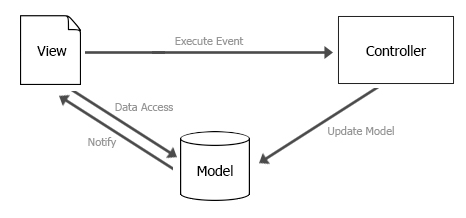
\includegraphics[scale=0.7]{Bilder/mvc.jpg}}
\end{figure}

\subsubsection{7-1 Pattern}
\label{sec:7-1}
Das \DesignPattern{7-1 Pattern}
\footnote{7-1 Pattern, \url{https://www.sass-guidelin.es/#architecture}} ist ein
Muster aus der Frontendarchitektur und definiert sich durch die Strukturierung des \ac{CSS} in 7 Ordner und
einer Hauptdatei. Grundsätzlich sind alle Teile des \ac{CSS} in 7 Ordnern
verteilt, und eine Datei (main.css) die alle Teilstücke importiert und zu einer Stylesheet kompiliert.
\begin{multicols}{4}
\begin{itemize}
\item abstracts/
\item base/
\item components/
\item layout/
\item pages/
\item themes/
\item vendors/
\item main.less
\end{itemize}
\end{multicols}
Die logische und modulare Trennung des \ac{CSS}-Codes verschafft eine klare
Übersicht für den Entwickler. Ebenso wird die Wiederverwendbarkeit von
Teilstücken verbessert und die Skalierbarkeit erhöht. Zusätzlich verschaft man
sich durch die Architektur eine Reihenfolge der Spezifität. Dieses zwingt einen
dazu Spitzen in der Spezifität von Selektoren zu vermeiden oder eher
am Ende des Stylesheets zu platzieren. So befindet sich im zweiten Ordner
"`base/"' nur \ac{CSS}, welches auschließlich HTML Standardelemente (\zB ul,
input,table, \usw) stilisiert. Der nächste Ordner besitzt immer eine höhere
Spezifität als der vorherige. In diesem Fall der Ordner "`components/"', der
bereits Klassen besitzt und aufgrund der höheren Spezifität den Style von
"`base/"' überschreiben kann.

\subsubsection{Block-Element-Modifier}
\label{sec:BEM}
\DesignPattern{Block-Element-Modifier} kurz \acs{BEM} ist ebenso eine moderne
Methode der Frontend-Architektur die erlaubt, Webprojekte modularer zu entwickeln.
Das erleichtert die Wartbarkeit und macht es Entwicklern einfacher, die
Codebasis jederzeit zu erweitern und trotzdem die Übersicht zu behalten.
Code wird in Blöcke und deren Elemente zerlegt, welche sich durch Modifikatoren
verändern lassen. Ein Block kann aus mehreren Elementen bestehen, welche durch
den Modifikator anpassbar sind. Durch dieses einfache Muster ist BEM der ideale
Weg, um im Team an Projekten mit sich ändernden Anforderungen zu arbeiten.
 \footnote{Vgl. t3n - Webdesign Magazin \cite{BEM}}
 
Die Methodik wird im Kapitel \ref{sec:BEMExample} anhand eines
praktischen Beispieles naherliegender erläutert.

\subsection{Entwurf der Benutzeroberfläche}
\label{sec:Benutzeroberflaeche} 
Das Screendesign wurde von einer externen Werbeagentur zur Verfügung gestellt.
Dementsprechend ist die Durchführung der Corporate Design Richtlinien durch \mh
überflüssig.
Der Screendesigner der \mh hat das Design lediglich in Slices \footnote{Geschnittenen Bilder/Grafiken} 
geschnitten und für die Entwicklung vorbereitet. Zur besseren Übersicht wurde
zusätzlich ein Wireframe gefertigt, welches im \Anhang{app:Entwuerfe}
begutachtet werden kann.

Um dem Entwickler eine bessere Übersicht der nötigen Styles zu bieten, hat der
Screendesigner einen Styleguide entworfen. Dies und weitere Oberflächen sind
ebenfalls unter \Anhang{app:Entwuerfe} zu finden.

\subsection{Pflichtenheft}
\label{sec:Pflichtenheft}
Mithilfe des Lastenheftes und den Erkenntnissen aus der Entwurfphase wurden
die Realisierungsvorgaben stichpunktartig erfasst. Ein Auszug davon ist im
\Anhang{app:Pflichtenheft} zu finden.

\usepackage{color}
\definecolor{lightgray}{rgb}{0.98, 0.98, 0.98}
\definecolor{darkgray}{rgb}{0.4, 0.4, 0.4}
%\definecolor{purple}{rgb}{0.65, 0.12, 0.82}
\definecolor{editorGray}{rgb}{0.95, 0.95, 0.95}
\definecolor{editorOcher}{rgb}{1, 0.5, 0} % #FF7F00 -> rgb(239, 169, 0)
\definecolor{editorGreen}{rgb}{0, 0.5, 0} % #007C00 -> rgb(0, 124, 0)
\definecolor{orange}{rgb}{1,0.45,0.13}		
\definecolor{olive}{rgb}{0.17,0.59,0.20}
\definecolor{brown}{rgb}{0.69,0.31,0.31}
\definecolor{purple}{rgb}{0.38,0.18,0.81}
\definecolor{lightblue}{rgb}{0.1,0.57,0.7}
\definecolor{lightred}{rgb}{1,0.4,0.5}
\usepackage{upquote}
\usepackage{listings}



% CSS
\lstdefinelanguage{CSS}{
  keywords={display,
  text-decoration,font-family,
  background-color,box-shadow,color,background-image:,margin,padding,font,weight,display,position,top,left,right,bottom,list,style,border,size,white,space,min,width,
  transition:, transform:, transition-property, transition-duration, transition-timing-function}, sensitive=true, morecomment=[l]{//}, morecomment=[s]{/*}{*/},
  morestring=[b]',
  morestring=[b]",
  alsoletter={:},
  alsodigit={-}
}

% JavaScript
\lstdefinelanguage{JavaScript}{
  morekeywords={typeof, new, true, false, catch, function, return, null, catch, switch, var, if, in, while, do, else, case, break},
  morecomment=[s]{/*}{*/},
  morecomment=[l]//,
  morestring=[b]",
  morestring=[b]'
}

\lstdefinelanguage{HTML5}{
  language=html,
  sensitive=true,	
  alsoletter={<>=-},	
  morecomment=[s]{<!-}{-->},
  tag=[s],
  otherkeywords={
  % General
  >,
  % Standard tags
	<!DOCTYPE,
  </html, <html, <head, <title, </title, <style, </style, <link, </head, <meta, />,
	% body
	</body, <body,
	% Divs
	</div, <div, </div>, 
	% Paragraphs
	</p, <p, </p>,
	% scripts
	</script, <script,
  % More tags...
  <canvas, /canvas>, <svg, <rect, <animateTransform, </rect>, </svg>, <video, <source, <iframe, </iframe>, </video>, <image, </image>, <header, </header, <article, </article
  },
  ndkeywords={
  % General
  =,
  % HTML attributes
  charset=, src=, id=, width=, height=, style=, type=, rel=, href=,
  % SVG attributes
  fill=, attributeName=, begin=, dur=, from=, to=, poster=, controls=, x=, y=, repeatCount=, xlink:href=,
  % properties
  margin:, padding:, background-color:, text-decoration:, color:, display:,
  box-shadow:, font-family:, width:, height:, background-image:, border:, top:,
  left:, position:, width:, height:, margin-top:, margin-bottom:, font-size:, line-height:,
	% CSS3 properties
  transform:, -moz-transform:, -webkit-transform:,
  animation:, -webkit-animation:,
  transition:,  transition-duration:, transition-property:, transition-timing-function:,
  }
}

\lstdefinestyle{htmlcssjs} {%
  % General design
%  backgroundcolor=\color{editorGray},
  basicstyle={\footnotesize\ttfamily},   
  frame=b,
  % line-numbers
  xleftmargin={0.75cm},
  numbers=left,
  stepnumber=1,
  firstnumber=1,
  numberfirstline=true,	
  % Code design
  identifierstyle=\color{black},
  keywordstyle=\color{blue}\bfseries,
  ndkeywordstyle=\color{editorGreen}\bfseries,
  stringstyle=\color{editorOcher}\ttfamily,
  commentstyle=\color{brown}\ttfamily,
  % Code
  language=HTML5,
  alsolanguage=JavaScript,
  alsodigit={.:;},	
  tabsize=2,
  showtabs=false,
  showspaces=false,
  showstringspaces=false,
  extendedchars=true,
  breaklines=true,
  % German umlauts
  literate=%
  {Ö}{{\"O}}1
  {Ä}{{\"A}}1
  {Ü}{{\"U}}1
  {ß}{{\ss}}1
  {ü}{{\"u}}1
  {ä}{{\"a}}1
  {ö}{{\"o}}1
}
%
\lstdefinestyle{py} {%
language=python,
literate=%
*{0}{{{\color{lightred}0}}}1
{1}{{{\color{lightred}1}}}1
{2}{{{\color{lightred}2}}}1
{3}{{{\color{lightred}3}}}1
{4}{{{\color{lightred}4}}}1
{5}{{{\color{lightred}5}}}1
{6}{{{\color{lightred}6}}}1
{7}{{{\color{lightred}7}}}1
{8}{{{\color{lightred}8}}}1
{9}{{{\color{lightred}9}}}1,
basicstyle=\footnotesize\ttfamily, % Standardschrift
numbers=left,               % Ort der Zeilennummern
%numberstyle=\tiny,          % Stil der Zeilennummern
%stepnumber=2,               % Abstand zwischen den Zeilennummern
numbersep=5pt,              % Abstand der Nummern zum Text
tabsize=4,                  % Groesse von Tabs
extendedchars=true,         %
breaklines=true,            % Zeilen werden Umgebrochen
keywordstyle=\color{blue}\bfseries,
frame=b,
commentstyle=\color{brown}\itshape,
stringstyle=\color{editorOcher}\ttfamily, % Farbe der String
showspaces=false,           % Leerzeichen anzeigen ?
showtabs=false,             % Tabs anzeigen ?
xleftmargin=17pt,
framexleftmargin=17pt,
framexrightmargin=5pt,
framexbottommargin=4pt,
%backgroundcolor=\color{lightgray},
showstringspaces=false,      % Leerzeichen in Strings anzeigen ?
}%
%

% !TEX root = ../Projektdokumentation.tex
\section{Implementierungsphase} 
\label{sec:Implementierungsphase}
Die Implementierung der Website geschieht in 3 Schritten: 
Die Entwicklung eines HTML Dummies unter Verwendung von \acs{HTML}5 und
\ac{CSS}3 \bzw  Less nach \acs{BEM} Methodik. Folgend die Ausarbeitung
der JavaScript \bzw jQuery Funktionalität im Frontend. Anschließend die Integration in 
das firmeneigene Content Management System \ct, sowie dessen Anpassung.

\subsection{Implementierung des HTML Dummys}
\label{sec:ImplementierungDummy}

Das die vertikale Darstellung der Elemente auf der Seite meistens mit der
Position im \ac{DOM} korrespondiert, wurde bei der Entwicklung des HTML Dummys
die Vorgehensweise Top-Bottom gewählt. Bei der Auswahl der \ac{HTML} Elemente
für die Container werden die semantischen \ac{HTML}5 Tags <article>, <section>,
<nav>, <aside>, \usw priorisiert. Der Einsatz von semantischen Tags steigert
die Suchmaschinenoptimierung und verbessert die \ac{DOM} Übersicht für den
Entwickler. \ac{W3C} schreibt vor, generische Container die nur für das Styling
gebraucht werden in Form von <div> Tags zu verwenden. Semantische Elemente sind
für relevante und bedeutsame Elemente aufzubewahren.


Das Top-Bottom Verfahren beruht sich auf die schrittweise Umsetzung der
\ac{HTML}-Seite in seperaten Blöcken. Aufgrund des angewandten Desktop
First Konzeptes, welches die Entstehung der Desktop Version als erstes vorsieht,
werden die Blöcke im nachhinein für die mobile Version mithilfe von Media
Queries optimiert. Zu beachten sind die in diesem Projekt benötigten Breakpoints für die
Desktopansicht, Tabletansicht und Smartphoneansicht. Unter Breakpoints versteht
man die Breite des Browserfensters in Pixel, von der die Position einzelner
Elemente abhängig sind. Die Pixelwerte dazu wurden unverändert von Bootstrap
übernommen. Eine grobe Strukur des \ac{DOM} ist im \Anhang{listing:DOM} zu
finden. 

\subsubsection{Umsetzung der BEM Methodik anhand eines Beispieles}
\label{sec:BEMExample}
Um den Code leserlicher und skalierbarer zu machen,
werden die Klassen in \acs{BEM} nach einem bestimmten Muster benannt. 
Die Konvention dazu ist \lstinline{.Block__Element--Modifier}. 
Bei der Umsetzung von \ac{BEM} ist ein umfangreiches Studieren der Screendesigns
unumgänglich. Dabei versucht man verschiedene Gestaltungselemente die sich
ähnlich sind (Varianten) zu einer Komponente zusammen zu fassen. 
Die Standardvariante ist meistens die, die am häufigsten vor kommt oder am
geringsten stilisiert wurde. 

Das in sich geschlossene Gestaltungselement wird als Block bezeichnet. 


\begin{figure}[ht]
\caption{Block}
\center{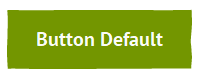
\includegraphics[scale=0.9]{Bilder/button-default.png}}
\end{figure}
\\
\begin{lstlisting}[style=htmlcssjs, backgroundcolor = \color{lightgray},
caption=BEM -- Block Default (HTML)] 
<a href="#" class="button">Button Default</a>
\end{lstlisting}

\begin{lstlisting}[style=htmlcssjs, backgroundcolor = \color{lightgray},
caption=BEM -- Block Default (CSS)]
.button {
  height: initial;
  position: relative;
  display: inline-block;
  padding: 15px 30px;
  font-size: 20px;
  color: @color-white;
  text-decoration: none;
  background-image: url('../img/svg/button.svg');
  [...]
}
\end{lstlisting}
\clearpage
Zur Veränderung der Optik werden Blöcke sowie Elemente mit Modifier ergänzt
(=Varianten).

\begin{figure}[ht]
\caption{Block mit Modifier}
\center{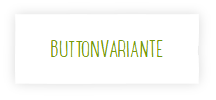
\includegraphics[scale=0.9]{Bilder/button-mod.png}}
\end{figure}

\begin{lstlisting}[style=htmlcssjs, backgroundcolor = \color{lightgray},
caption=BEM -- Block mit Modifier (HTML)]
<a href="#" class="button button--white">Buttonvariante</a>
\end{lstlisting}

\begin{lstlisting}[style=htmlcssjs, backgroundcolor = \color{lightgray},
caption=BEM -- Modifier (CSS)] 
.button--white {
  background-color: white;
  padding: 37px 50px 31px 50px;
  font-family: @font-LunchBox-Light;
  color: @color-primary;
  box-shadow: 0px 0px 10px 0px rgba(0,0,0,0.2);
}

\end{lstlisting}

Die Elemente innerhalb eines Blockes werden simpel als Elemente bezeichnet.

\begin{figure}[ht]
\caption{Block mit Element}
\center{
\includegraphics[scale=0.9]{Bilder/button-elem.png}}
\end{figure}

\begin{lstlisting}[style=htmlcssjs, backgroundcolor = \color{lightgray},
caption=BEM -- Block mit Element (HTML)]
<a href="#" class="button button--white">
	<i class="button__icon button__icon--facebook"></i>
	Gefällt mir
</a>
\end{lstlisting}

\begin{lstlisting}[style=htmlcssjs, backgroundcolor = \color{lightgray},
caption=BEM -- Element (CSS)]
.button__icon {
  background-image: url('../img/svg/fb-icon.svg');
  width:24px;
  height:24px;
}
\end{lstlisting}


\subsection{Implementierung der Javascript Funktionalitäten}
\label{sec:ImplementierungJS}
Durch das Scrollen nach unten verkleinert sich das Logo soweit, so dass das
Logo  den weißen Bereich (Navbar) nicht überschreitet. Dies wird mit dem
Hinzufügen einer Element-Modifier Klasse \\
(\lstinline{.navbar__brand--minimized}) bewerkstelligt.
\\
\begin{lstlisting}[style=htmlcssjs, backgroundcolor = \color{lightgray},
caption=Logominimierung beim Scrollen]
    $(document).scroll(function () {
        if ($(document).scrollTop() > 0) {
            $('.navbar__brand').addClass('navbar__brand--minimized');
        } else {
            $('.navbar__brand').removeClass('navbar__brand--minimized');
        }
     }).trigger("scroll");     
\end{lstlisting}

Ein Eventhandler wird an das Scroll-Event des Window-Objekts gebunden.
Wenn die Scrollposition größer gleich der oberen Kante des Browserfensters ist
(>0px), wird dem Logo die Klasse \lstinline{.navbar__brand--minimized}
hinzugefügt. Ansonsten wird diese Klasse im Else-Zweig entfernt.
Die Klasse selber beinhaltet Styles zur animierten Skalierung des Logos.

Bei der Navigation wurde aufgrund seiner hohen Komplexität, auf die schon
fertige Dropdownfunktion des Frameworks Bootsrap verzichtet. Ein weiteres
Problem ist, dass die Bootstrap Funktionalität keine Möglichkeit eines
Subdropdowns unterstützt. Das Skript dazu ist im \Anhang{app:Dropdown} zu
finden.

\subsection{Implementierung des Content Management System}
\label{sec:ImplementierungCMS}

Nach der vollständigen Umsetzung des \ac{HTML} Dummys mit rein statischen
Testinhalt beginnt die Integration des \ac{CMS}. Die \mh setzt auf die
firmeninterne Lösung conTRANCE v6. Der erste Schritt ist der Pull \bzw Export
des letzten conTRANCE Releases aus GIT. Die Dateien des HTML Dummys werden
in die conTRANCE Dateienstruktur aufgenommen. Die Datenbanktabellen des
\ac{CMS} werden vom Enticklungsserver kopiert und in eine für das Projekt neu
angelegte Datenbank importiert. Alle Inhaltsbezogenen Tabelle werden geleert
und die Datenbankanbindung wird mit entsprechenden Daten konfiguriert.
Anschließend kann über das Backend ein rudimentärer Navigationsbaum angelegt
werden, welcher für die weitere Umsetzung notwendig ist. Nun werden die Ausgaben
aus dem \ac{CMS} zum Style des Screendesigns angegleicht.

Da \ct schon alle Anforderungen des Kunden erfüllt, waren dessen Anpassungen,
die nur die visuelle Ausgabe betreffen, nicht beachtenswert.

\subsection{Testphase}
\label{sec:Testphase}
Zur Überprüfung von Darstellungsfehlern wird im Laufe der
Implementierungsphase die Ausgabe aller relevanten Browser in allen nötigen
Darstellungsgrößen kontrolliert. Dazu besteht eine laufende \\ Kommunikation
zwischen Entwickler, dem Projektmanagement und dem Screendesigner im Hause, der
alle Slices vom Screendesign bereit stellt.
Für Schriftgrößen und Abstände wird die relative Maßeinheit "`rem"' eingesetzt.
Diese Einheit orientiert sich an den Schriftgrößenwert des HTML
Rootelements (<html>). Um eine richtige proportionale Darstellung je nach
Browsereinstellungen zu gewährleisten, wird der Schriftgröße des Rootelements
ein prozentualer Wert zugewiesen. Im Hinblick darauf, dass jeder Browser im
Desktop und mobilen Bereich eine Standarteinstellung von 16px Schriftgröße
besitzt, wird der prozentuale Wert -- bei einem Beispiel von 18px
Fließtextgröße -- auf 112,5\% (18 * 100 / 16) gesetzt. Dies bewirkt eine
proportionale Skalierung von Abständen und Schriftgrößen im Falle von
benutzerdefinierten Browsereinstellungen.

\Zwischenstand{Implementierungsphase}{Implementierung}

% !TEX root = ../Projektdokumentation.tex
\section{Projektabschluss} 
\label{sec:Projektabschluss}

\subsection{Abnahme} 
\label{sec:Abnahme}
Während der Abnahmephase wurde das Projekt in die Zielumgebung eingeführt und
nochmals nach Darstellungsfehler untersucht. Währenddessen füllt das
Projektmanagement die Website mit dem endgültigen Content. Zusätzlich wurde der
Mitarbeiter des Projektmanagments auf Besonderheiten und Backendabläufe
hingewiesen. Diese gibt er dem Kunden im Form einer Schulung kund.

\subsection{Soll-/Ist-Vergleich}
\label{sec:SollIstVergleich}

Zurückschauend, ist es es zu bemerken, dass etwas mehr Zeit gebraucht wurde,
als im zuvor unter \xx Kapitel festgelegten Zeitplan zu sehen ist. Dennoch
zeigte der Ku
\begin{itemize}
	\item Wurde das Projektziel erreicht und wenn nein, warum nicht?
	\item Ist der Auftraggeber mit dem Projektergebnis zufrieden und wenn nein, warum nicht?
	\item Wurde die Projektplanung (Zeit, Kosten, Personal, Sachmittel) eingehalten oder haben sich Abweichungen ergeben und wenn ja, warum?
	\item Hinweis: Die Projektplanung muss nicht strikt eingehalten werden. Vielmehr sind Abweichungen sogar als normal anzusehen. Sie müssen nur vernünftig begründet werden (\zB durch Änderungen an den Anforderungen, unter-/überschätzter Aufwand).
\end{itemize}

\paragraph{Beispiel (verkürzt)}
Wie in Tabelle~\ref{tab:Vergleich} zu erkennen ist, konnte die Zeitplanung bis auf wenige Ausnahmen eingehalten werden.
\tabelle{Soll-/Ist-Vergleich}{tab:Vergleich}{Zeitnachher.tex}

\subsection{Dokumentation}
\label{sec:Dokumentation}

\begin{itemize}
	\item Wie wurde die Anwendung für die Benutzer/Administratoren/Entwickler dokumentiert (\zB Benutzerhandbuch, \acs{API}-Dokumentation)?
	\item Hinweis: Je nach Zielgruppe gelten bestimmte Anforderungen für die Dokumentation (\zB keine IT-Fachbegriffe in einer Anwenderdokumentation verwenden, aber auf jeden Fall in einer Dokumentation für den IT-Bereich).
\end{itemize}

\paragraph{Beispiel}
Ein Ausschnitt aus der erstellten Benutzerdokumentation befindet sich im \Anhang{app:BenutzerDoku}.
Die Entwicklerdokumentation wurde mittels PHPDoc\footnote{Vgl. \cite{phpDoc}} automatisch generiert. Ein beispielhafter Auszug aus der Dokumentation einer Klasse findet sich im \Anhang{app:Doc}. 

\Zwischenstand{Dokumentation}{Dokumentation}



\subsection{Fazit} 
\label{sec:Fazit}






\begin{itemize}
	\item Was hat der Prüfling bei der Durchführung des Projekts gelernt (\zB Zeitplanung, Vorteile der eingesetzten Frameworks, Änderungen der Anforderungen)?
\end{itemize}



\begin{itemize}
	\item Wie wird sich das Projekt in Zukunft weiterentwickeln (\zB geplante Erweiterungen)?
\end{itemize}




% !TEX root = ../Projektdokumentation.tex
\section{Einführungsphase}
\label{sec:Einfuehrungsphase}

\begin{itemize}
	\item Welche Schritte waren zum Deployment der Anwendung nötig und wie wurden sie durchgeführt (automatisiert/manuell)?
	\item Wurden \ggfs Altdaten migriert und wenn ja, wie?
	\item Wurden Benutzerschulungen durchgeführt und wenn ja, Wie wurden sie vorbereitet?
\end{itemize}


\Zwischenstand{Einführungsphase}{Einfuehrung}

% !TEX root = ../Projektdokumentation.tex
\section{Dokumentation}
\label{sec:Dokumentation}

\begin{itemize}
	\item Wie wurde die Anwendung für die Benutzer/Administratoren/Entwickler dokumentiert (\zB Benutzerhandbuch, \acs{API}-Dokumentation)?
	\item Hinweis: Je nach Zielgruppe gelten bestimmte Anforderungen für die Dokumentation (\zB keine IT-Fachbegriffe in einer Anwenderdokumentation verwenden, aber auf jeden Fall in einer Dokumentation für den IT-Bereich).
\end{itemize}

\paragraph{Beispiel}
Ein Ausschnitt aus der erstellten Benutzerdokumentation befindet sich im \Anhang{app:BenutzerDoku}.
Die Entwicklerdokumentation wurde mittels PHPDoc\footnote{Vgl. \cite{phpDoc}} automatisch generiert. Ein beispielhafter Auszug aus der Dokumentation einer Klasse findet sich im \Anhang{app:Doc}. 

\Zwischenstand{Dokumentation}{Dokumentation}

% !TEX root = ../Projektdokumentation.tex


% Literatur ------------------------------------------------------------------
\clearpage
\renewcommand{\refname}{Literaturverzeichnis}
\bibliography{Bibliographie}
\bibliographystyle{Allgemein/natdin} % DIN-Stil des Literaturverzeichnisses
% !TEX root = Projektdokumentation.tex
\clearpage
\addsec{Eidesstattliche Erklärung}

% Hinweis: die eidesstattliche Erklärung ist ggfs. an die Richtlinie der IHK anzupassen

Ich, \autorName, versichere hiermit, dass ich meine \textbf{\betreff} mit dem
Thema
\begin{quote}
\textit{\kompletterTitel}
\end{quote}
selbständig verfasst und keine anderen als die angegebenen Quellen und Hilfsmittel benutzt habe,
wobei ich alle wörtlichen und sinngemäßen Zitate als solche gekennzeichnet habe. Die Arbeit
wurde bisher keiner anderen Prüfungsbehörde vorgelegt und auch nicht veröffentlicht.\\[6ex]

\abgabeOrt, den \abgabeTermin


\rule[-0.2cm]{5.5cm}{0.5pt}

\textsc{\autorName}


% Anhang ---------------------------------------------------------------------
\clearpage
\appendix
\pagenumbering{roman}
% !TEX root = Projektdokumentation.tex
\section{Anhang}
\subsection{Detaillierte Zeitplanung}
\label{app:Zeitplanung}

\tabelleAnhang{ZeitplanungKomplett}

\subsection{Verwendete Ressourcen}
\label{list:Ressourcenplanung}

\paragraph{Hardware}
\begin{itemize}
	\item Bürarbeitsplatz
	\item Rechner
	\item Zwei 21' Monitore
\end{itemize}

\paragraph{Software}
\begin{itemize}
	\item Linux Xubuntu 16.04.2 LTS Kernel 4.8.0 -- Bestriebssystem
	\item GIT -- Werkzeug zur Versionsverwaltung
	\item Node.js -- Plattform zur Komplilierung der LESS Dateien
	\item jQuery -- freie Javascript-Bibliothek	
	\item phpMyAdmin -- Webapplikation zur Administration von MySQL
	\item Filezilla 3.15.0.2 -- Werkzeug zur Dateiübertragung
	\item Enterprise Architect –- Werkzeug zur Erstellung von Modellen und
	Diagrammen
	\item MiKTeX -- LaTeX Implemmentierung unter Windows
	\item Eclipse Neon -- \ac{IDE} (mit Texlipse)
	\item VirtualBox -- Virtualisierungssoftware für Betriebssysteme (Windows
	10)

\end{itemize}

\paragraph{Personal}
\begin{itemize}
	\item Projektleiter -- Festlegung der Anforderungen und Abnahme des Projektes

	\item Fachbereichsleiter -- Festlegung der Anforderungen und Abnahme des
	Projektes
	\item Screendesigner -- Stellt die grafische Grundlage zur Verfügung
	\item Anwendungsentwickler -- Projektumsetzung
\end{itemize}
\clearpage

\label{app:Lastenheft}
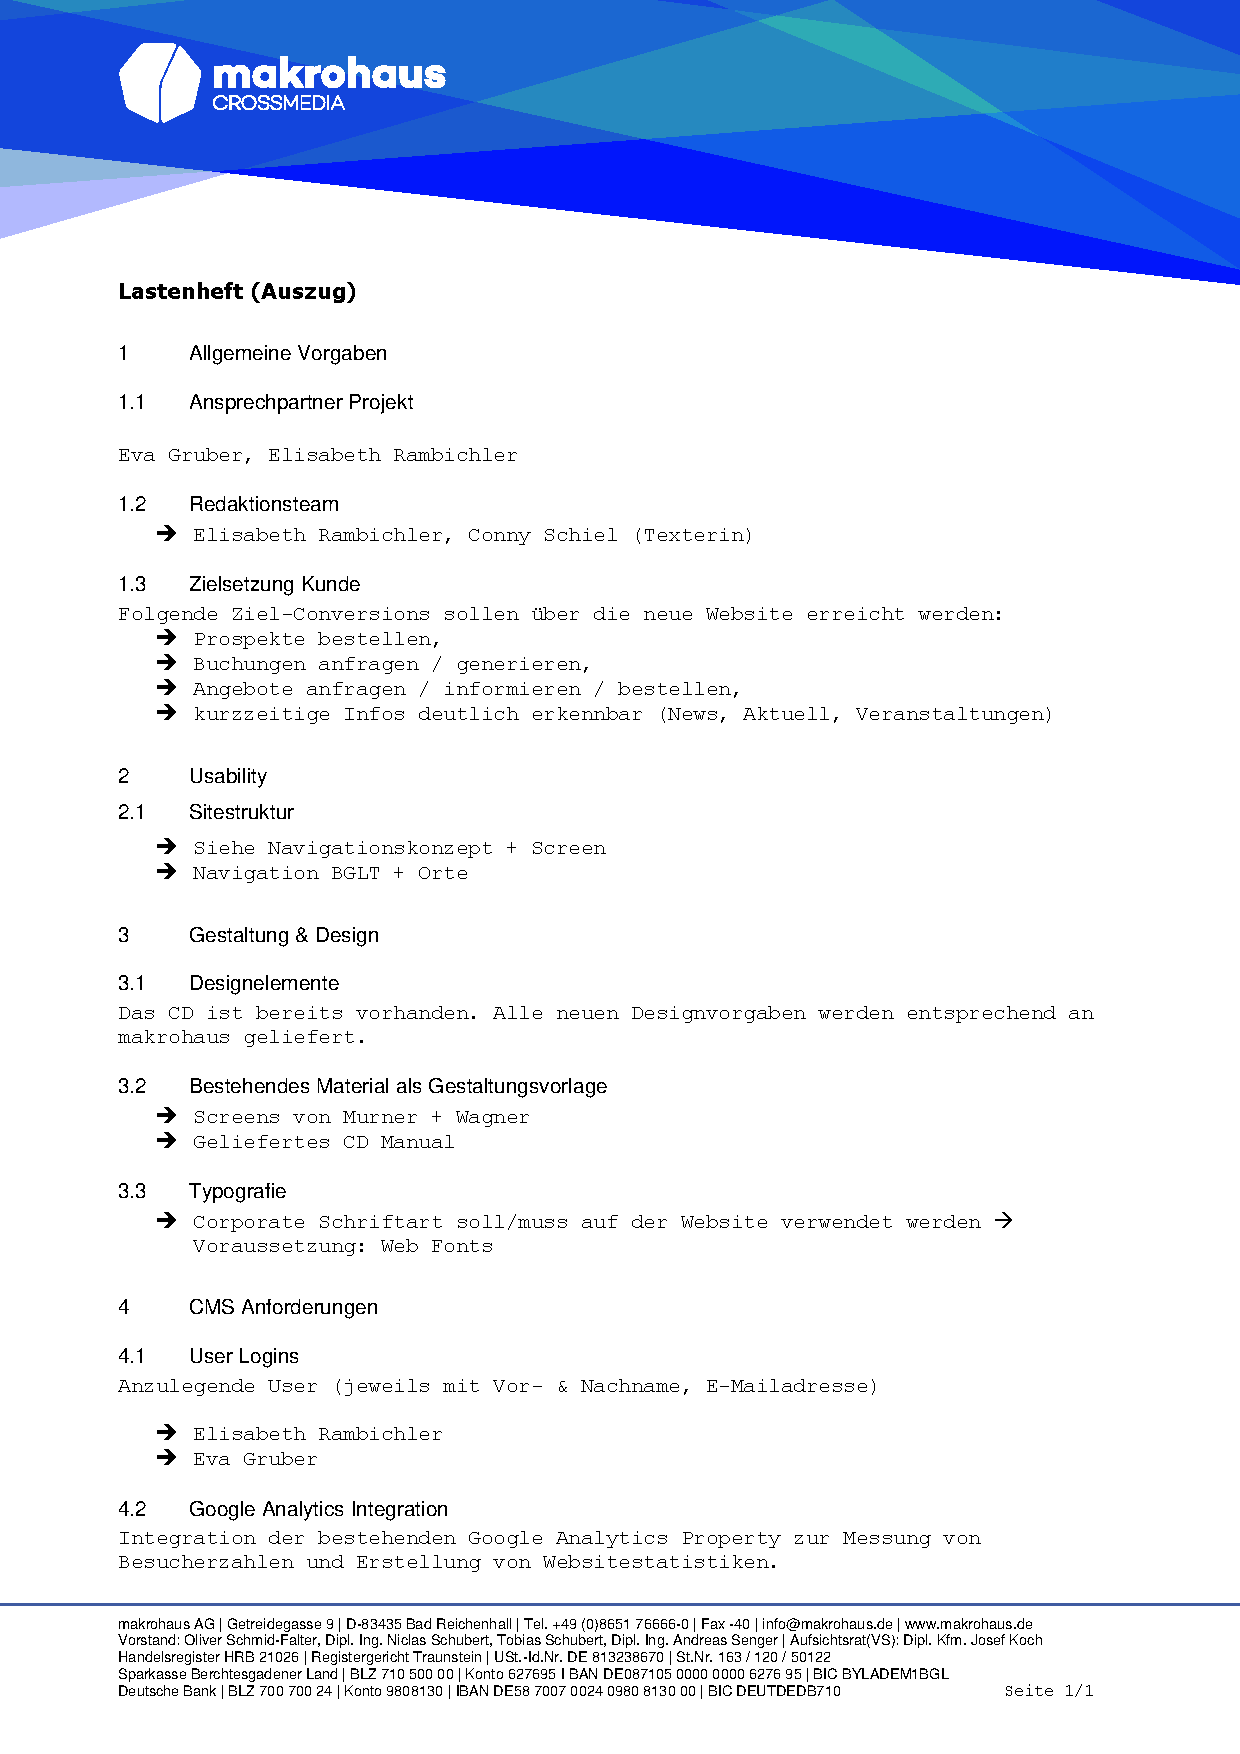
\includepdf{Anhang/Grobkonzept.pdf}
\clearpage

\subsection{Use-Case-Diagramm}
\label{app:UseCase}
\begin{figure}[htb]
\centering
\includegraphicsKeepAspectRatio{Bilder/waging-usecase.jpg}{0.9}
\caption{Website Use-Case-Diagramm}
\end{figure}

\subsection{Pflichtenheft (Auszug)}
\label{app:Pflichtenheft}

\subsubsection*{Zielbestimmung}

\begin{enumerate}[itemsep=0em,partopsep=0em,parsep=0em,topsep=0em]
\item Musskriterien % Wikipedia: für das Produkt unabdingbare Leistungen, die in jedem Fall erfüllt werden müssen
	\begin{enumerate}
	\item Modul-Liste: Zeigt eine filterbare Liste der Module mit den dazugehörigen Kerninformationen sowie Symbolen zur Einhaltung des Entwicklungsprozesses an
		\begin{itemize}
		\item In der Liste wird der Name, die Bibliothek und Daten zum Source und Kompilat eines Moduls angezeigt.
		\item Ebenfalls wird der Status des Moduls hinsichtlich Source und Kompilat angezeigt. Dazu gibt es unterschiedliche Status-Zeichen, welche symbolisieren in wie weit der Entwicklungsprozess eingehalten wurde \bzw welche Schritte als nächstes getan werden müssen. So gibt es \zB Zeichen für das Einhalten oder Verletzen des Prozesses oder den Hinweis auf den nächsten zu tätigenden Schritt. 
		\item Weiterhin werden die Benutzer und Zeitpunkte der aktuellen Version der Sourcen und Kompilate angezeigt. Dazu kann vorher ausgewählt werden, von welcher Umgebung diese Daten gelesen werden sollen. 
		\item Es kann eine Filterung nach allen angezeigten Daten vorgenommen werden. Die Daten zu den Sourcen sind historisiert. Durch die Filterung ist es möglich, auch Module zu finden, die in der Zwischenzeit schon von einem anderen Benutzer editiert wurden.
		\end{itemize}
	\item Tag-Liste: Bietet die Möglichkeit die Module anhand von Tags zu filtern. 
		\begin{itemize}
		\item Es sollen die Tags angezeigt werden, nach denen bereits gefiltert wird und die, die noch der Filterung hinzugefügt werden könnten, ohne dass die Ergebnisliste leer wird.
		\item Zusätzlich sollen die Module angezeigt werden, die den Filterkriterien entsprechen. Sollten die Filterkriterien leer sein, werden nur die Module angezeigt, welche mit einem Tag versehen sind.
		\end{itemize}
	\item Import der Moduldaten aus einer bereitgestellten \acs{CSV}-Datei
		\begin{itemize}
		\item Es wird täglich eine Datei mit den Daten der aktuellen Module erstellt. Diese Datei wird (durch einen Cronjob) automatisch nachts importiert.
		\item Dabei wird für jedes importierte Modul ein Zeitstempel aktualisiert, damit festgestellt werden kann, wenn ein Modul gelöscht wurde.
		\item Die Datei enthält die Namen der Umgebung, der Bibliothek und des Moduls, den Programmtyp, den Benutzer und Zeitpunkt des Sourcecodes sowie des Kompilats und den Hash des Sourcecodes.
		\item Sollte sich ein Modul verändert haben, werden die entsprechenden Daten in der Datenbank aktualisiert. Die Veränderungen am Source werden dabei aber nicht ersetzt, sondern historisiert.
		\end{itemize}
	\item Import der Informationen aus \ac{SVN}. Durch einen \gqq{post-commit-hook} wird nach jedem Einchecken eines Moduls ein \acs{PHP}-Script auf der Konsole aufgerufen, welches die Informationen, die vom \ac{SVN}-Kommandozeilentool geliefert werden, an \acs{NatInfo} übergibt.
	\item Parsen der Sourcen
		\begin{itemize}
		\item Die Sourcen der Entwicklungsumgebung werden nach Tags, Links zu Artikeln im Wiki und Programmbeschreibungen durchsucht.
		\item Diese Daten werden dann entsprechend angelegt, aktualisiert oder nicht mehr gesetzte Tags/Wikiartikel entfernt.
		\end{itemize}
	\item Sonstiges
		\begin{itemize}
		\item Das Programm läuft als Webanwendung im Intranet.
		\item Die Anwendung soll möglichst leicht erweiterbar sein und auch von anderen Entwicklungsprozessen ausgehen können.
		\item Eine Konfiguration soll möglichst in zentralen Konfigurationsdateien erfolgen.
		\end{itemize}
	\end{enumerate}
\end{enumerate}

\subsubsection*{Produkteinsatz}

\begin{enumerate}[itemsep=0em,partopsep=0em,parsep=0em,topsep=0em]
\item{Anwendungsbereiche\\
Die Webanwendung dient als Anlaufstelle für die Entwicklung. Dort sind alle Informationen für die Module an einer Stelle gesammelt. Vorher getrennte Anwendungen werden ersetzt \bzw verlinkt.}
\item{Zielgruppen\\
\NI wird lediglich von den \ac{Natural}-Entwicklern in der EDV-Abteilung genutzt.}
\item{Betriebsbedingungen\\ % Wikipedia: physikalische Umgebung des Systems, tägliche Betriebszeit, ständige Beobachtung des Systems durch Bediener oder unbeaufsichtigter Betrieb
Die nötigen Betriebsbedingungen, also der Webserver, die Datenbank, die Versionsverwaltung, das Wiki und der nächtliche Export sind bereits vorhanden und konfiguriert. Durch einen täglichen Cronjob werden entsprechende Daten aktualisiert, die Webanwendung ist jederzeit aus dem Intranet heraus erreichbar.}
\end{enumerate}


%\subsection{Datenbankmodell}
%\label{app:Datenbankmodell}
%ER-Modelle kann man auch direkt mit \LaTeX{} zeichnen, siehe \zB
% \url{http://www.texample.net/tikz/examples/entity-relationship-diagram/}.
%\begin{figure}[htb]
%\centering
%\includegraphicsKeepAspectRatio{database.pdf}{1}
%\caption{Datenbankmodell}
%\end{figure}
%\clearpage

\subsection{Oberflächenentwürfe}
\label{app:Entwuerfe}

\begin{figure}[h]
\centering
\includegraphicsKeepAspectRatio{Bilder/mh-wireframe.jpg}{0.74}
\caption{Wireframe der Startseite}
\end{figure}

\begin{figure}[h]
\centering
\includegraphicsKeepAspectRatio{Bilder/mh-style-template.jpg}{1}
\caption{Übersicht von relevanten Styles}
\end{figure}



\clearpage
\subsection{Screenshots der Anwendung}
\label{Screenshots}

\begin{figure}[h]
\centering
\includegraphicsKeepAspectRatio{Bilder/mh-start.jpg}{0.7}
\caption{Screendesign: Startseite Desktop-Ansicht}
\end{figure}


\begin{figure}[h]
\centering
\includegraphicsKeepAspectRatio{Bilder/mh-start-xs.jpg}{1}
\caption{Screendesign: Startseite Mobil-Ansicht}
\end{figure}

\begin{figure}[h]
\centering
\includegraphicsKeepAspectRatio{Bilder/mh-nav.png}{1}
\caption{Navigation}
\end{figure}

\clearpage

\clearpage
\subsection{Grobstruktur -- Document Object Model}
\label{listing:DOM}
\begin{lstlisting}[style=htmlcssjs, backgroundcolor = \color{lightgray},
caption=DOM der index.php] 
<!DOCTYPE>
<html> 
	<head>
	    <meta charset="utf-8">
	    <meta http-equiv="X-UA-Compatible" content="IE=edge,chrome=1">
	    <meta name="viewport" content="width=device-width, initial-scale=1">
	    {Einbettung von Javascript Ressourcen}
	    {Einbettung der ShareIcons und Favicon}
	</head>
	
	<body>
	
	<header>
	    {Einbettung der Navigation}
	    <div class="header__slider">
	        {Einbettung der Slideshow}
	    </div>
	</header>
	
	<aside>
	    {Einbettung der Sidebar}
	</aside>
	
	<main id="content">
	    {Einbettung Breadcrumb Navigation}
	    <div class="container">
	        <section class="row">
	            {Einbettung Breadcrumb Navigation}
	        </section>
	    </div>
	</main>
	
	<footer class="footer">
	    {Einbettung Footer}
	</footer>
	
	{Einbettung von Javascript Ressourcen}
	
	</body>	
</html>
\end{lstlisting}
\clearpage
\clearpage
\subsection{Dropdownfunktionalität der Navigation}
\label{app:Dropdown}
\begin{lstlisting}[style=htmlcssjs, backgroundcolor = \color{lightgray},
caption=Javascript Dropdownfunktionalität]
    // Toggle Button zum Aufklappen der Navigation in der mobilen Ansicht    
    var menu = $('.menu-main'),
        menuToggleBtn = $('[data-target="menu"]'),
        logo = $(".navbar__brand");

    menuToggleBtn.click(function () {
        $(this).hide();
        $(this).siblings('.menu__link--toggle').css({display: "block"});
        logo.animate({opacity: 0}, 100);
        menu.slideToggle(300, function () {
            if (menu.css("display") == "none") {
                logo.stop().animate({opacity: 1}, 200);
            }
        });
    });
    
    //DopDown Funktionalität
    var dropdown_link = $('[data-toggle="dropdown"]'),
        sub_dropdown_link = $('[data-toggle="sub-dropdown"]'); 
         
    // Primary-Dropdown
    dropdown_link.on('click', function (e) {
        e.stopPropagation();
        dropdown_container = $(this).siblings('.menu__dropdown-container');
        dropdown_container.slideToggle(toggleTime);
        //* andere Conteiner einklappen lassen *//
        $('.menu__dropdown-container').not(dropdown_container).not($('.menu__dropdown-container--sub')).slideUp(slideUpTime);
    });     
         
    // Sub-Dropdown
    sub_dropdown_link.on('click', function (e) {
        e.stopPropagation();
        $this = $(this);
        sub_dropdown_link.not($this).html('+').removeClass('minus');
        $this.toggleClass('minus');
        if ($this.hasClass('minus')) {
            $this.html('-')
        } else {
            $this.html('+')
        } 
        dropdown_container = $this.siblings('.menu__dropdown-container--sub');
        dropdown_container.slideToggle(toggleTime);
        //* andere Container einklappen lassen *//
        $('.menu__dropdown-container--sub').not(dropdown_container).slideUp(slideUpTime);
    });


    /* Anything that gets to the document
     will hide the dropdown */
    $(document).click(function () {
        $(".menu__dropdown-container").css('display', 'none');
    });

    /* Clicks within the dropdown won't make
     it past the dropdown itself */
    $(".menu__dropdown-container:not('button')").click(function (e) {
        elementClassName = e.target.className;
        if (e.target.className.search('search-housing__submit') == -1) {
            e.stopPropagation();
        }
    });
    
\end{lstlisting}

%\subsection{Entwicklerdokumentation}
\label{app:Doc}
\begin{center}
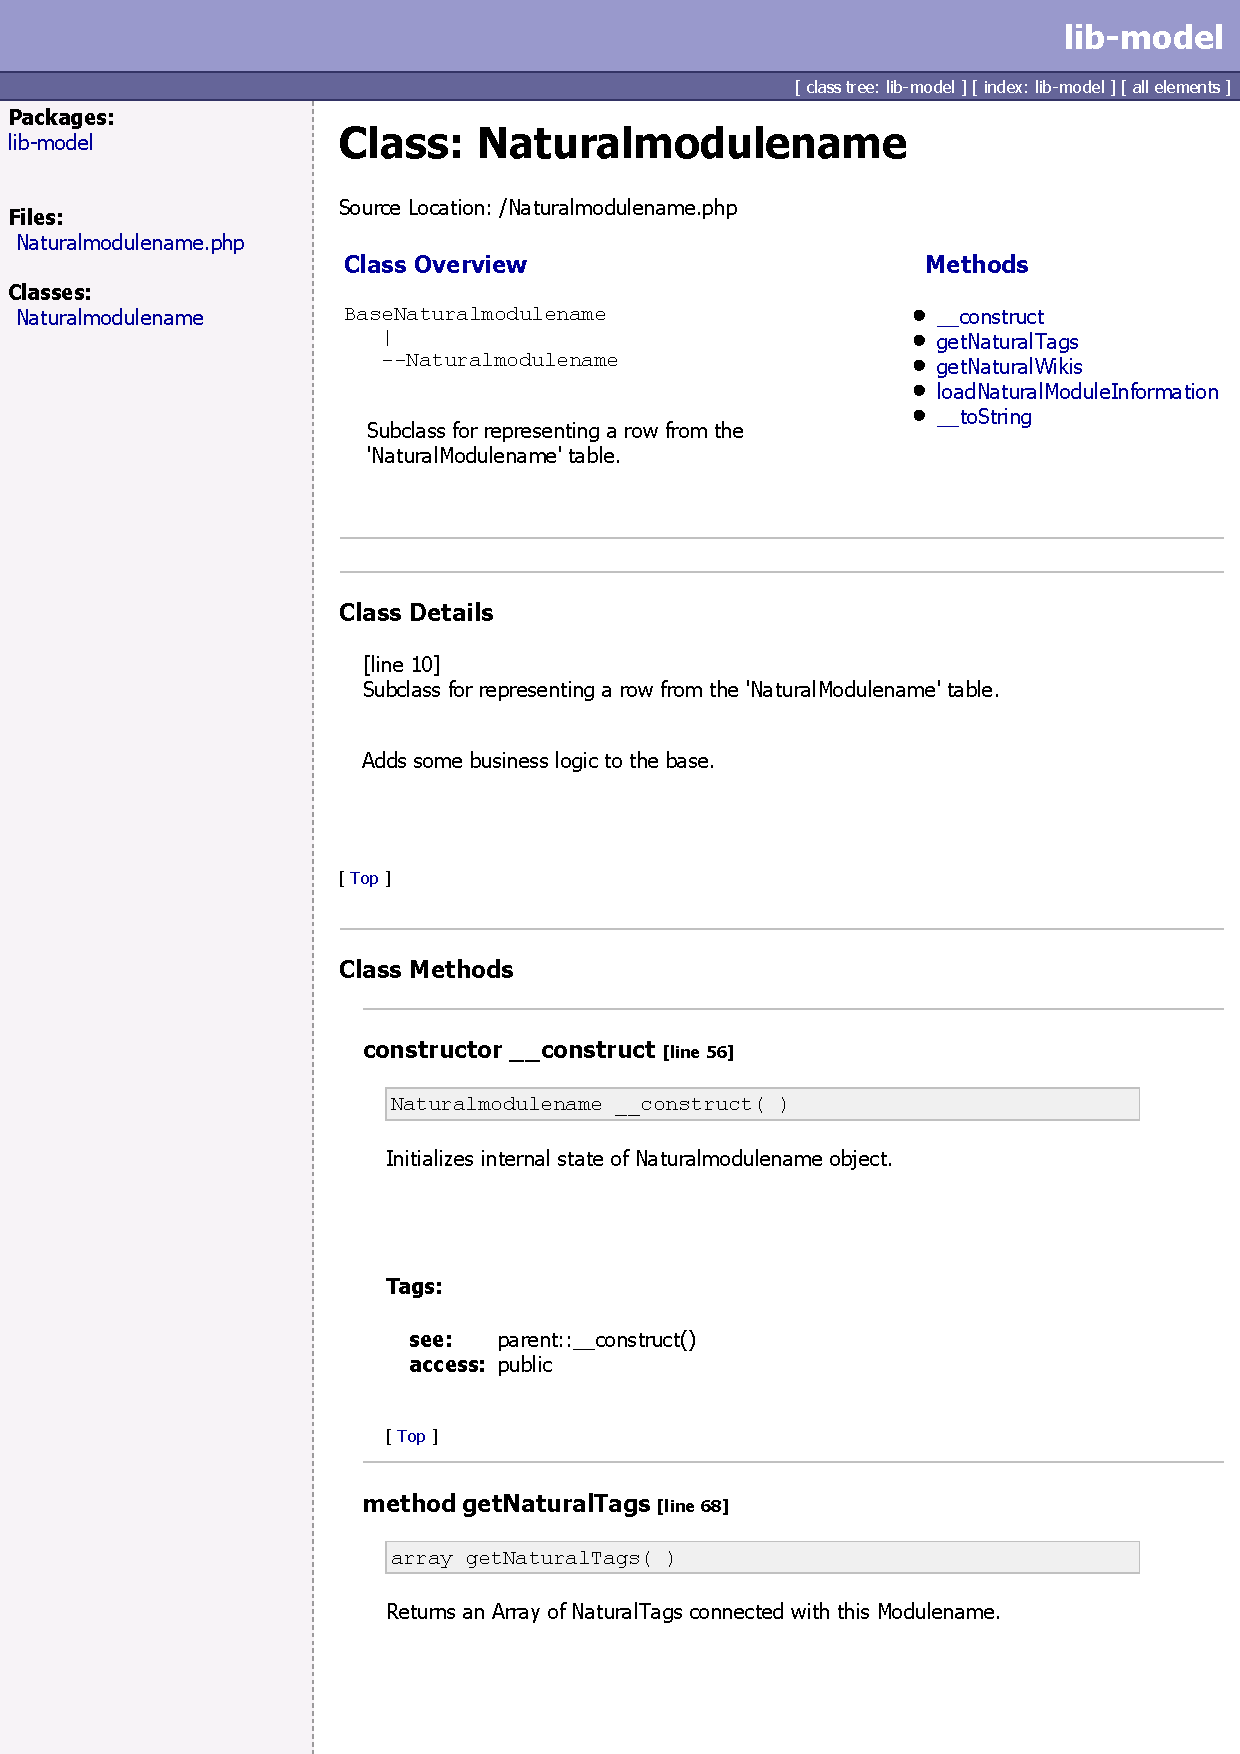
\includegraphics[page=1, width=0.9\textwidth]{doc.pdf}

\includegraphics[page=2, width=0.9\textwidth]{doc.pdf}
\end{center}

%\clearpage
%\subsection{Testfall und sein Aufruf auf der Konsole}
\label{app:Test}
\lstinputlisting[language=php]{Listings/tests.php}
\clearpage
\begin{figure}[htb]
\centering
\includegraphicsKeepAspectRatio{testcase.jpg}{1}
\caption{Aufruf des Testfalls auf der Konsole}
\end{figure}


%\subsection{Klasse: ComparedNaturalModuleInformation}
%\label{app:CNMI}
%Kommentare und simple Getter/Setter werden nicht angezeigt.
%\lstinputlisting[language=php]{Listings/cnmi.php}
%\clearpage

%\subsection{Klassendiagramm}
%\label{app:Klassendiagramm}
%Klassendiagramme und weitere \acs{UML}-Diagramme kann man auch direkt mit
% \LaTeX{} zeichnen, siehe \zB \url{http://metauml.sourceforge.net/old/class-diagram.html}.
%\begin{figure}[htb]
%\centering
%\includegraphicsKeepAspectRatio{Klassendiagramm.pdf}{1}
%\caption{Klassendiagramm}
%\end{figure}
%\clearpage

%\subsection{Benutzerdokumentation}
\label{app:BenutzerDoku}
Ausschnitt aus der Benutzerdokumentation:

\begin{table}[htb]
\begin{tabularx}{\textwidth}{cXX}
\rowcolor{heading}\textbf{Symbol} & \textbf{Bedeutung global} & \textbf{Bedeutung einzeln} \\
\includegraphicstotab[]{weather-clear.png} & Alle Module weisen den gleichen Stand auf. & Das Modul ist auf dem gleichen Stand wie das Modul auf der vorherigen Umgebung. \\
\rowcolor{odd}\includegraphicstotab[]{weather-clear-night.png} & Es existieren keine Module (fachlich nicht möglich). & Weder auf der aktuellen noch auf der vorherigen Umgebung sind Module angelegt. Es kann also auch nichts übertragen werden. \\
\includegraphicstotab[]{weather-few-clouds-night.png} & Ein Modul muss durch das Übertragen von der vorherigen Umgebung erstellt werden. & Das Modul der vorherigen Umgebung kann übertragen werden, auf dieser Umgebung ist noch kein Modul vorhanden. \\
\rowcolor{odd}\includegraphicstotab[]{weather-few-clouds.png} & Auf einer vorherigen Umgebung gibt es ein Modul, welches übertragen werden kann, um das nächste zu aktualisieren. & Das Modul der vorherigen Umgebung kann übertragen werden um dieses zu aktualisieren. \\
\includegraphicstotab[]{weather-storm.png} & Ein Modul auf einer Umgebung wurde entgegen des Entwicklungsprozesses gespeichert. & Das aktuelle Modul ist neuer als das Modul auf der vorherigen Umgebung oder die vorherige Umgebung wurde übersprungen. \\
\end{tabularx}
\end{table}




\end{document}
